\chapter{Querying the Semantic Web -- SPARQL}
\label{ch6}

RDF provides a simple way to represent distributed data. The triple is
the simplest way to represent a named connection between two things. But
a representation of data is useless without some means of accessing that
data. The standard way to access RDF data uses a query language called
SPARQL. SPARQL stands for SPARQL Protocol And RDF Query Language (yes,
the ``S'' in ``SPARQL'' stands for ``SPARQL,'' sigh). The SPARQL query
language works closely with the structure of RDF itself. SPARQL query
patterns are represented in a variant of Turtle (the same language that
we use to express RDF throughout this book). The queried RDF graph can be created from one
kind of data or merged from many; in either case, SPARQL is the way to
query it.

This chapter gives examples of the SPARQL query language. Most of the
examples are based on version 1.0 of the standard, released in 2008. More advanced features 
are now available in the more recent SPARQL 1.1 release.  SPARQL 1.1 is backward compatible with
SPARQL 1.0, so the basic features are available for both releases. 

SPARQL is a query language and shares many features with other query
languages like XQUERY and SQL. But it differs from each of these query
languages in important ways (as they differ from one another). Since we
don't want to assume that a reader has a background in any specific
query language (or even query languages at all), we begin with a gentle
introduction to querying data. We start with the most basic information
retrieval system, which we call a Tell-and- Ask system.

\section{Tell-And-Ask Systems}

A Tell-and-Ask system is a simple system -- you tell it some facts, and
then it can answer questions you ask based on what you told it. Consider the following simple example:

\textbf{Tell:} James Dean played in the movie \emph{Giant}. Then you could ask
questions like:

\textbf{Ask:} Who played in \emph{Giant}?

\textbf{Answer:} James Dean

\textbf{Ask:} James Dean played in what?

\textbf{Answer:} ``\emph{Giant}

You might tell it some more things, too, like:

\textbf{Tell:} James Dean played in \emph{East of Eden}. 
\textbf{Tell:} James Dean played in \emph{Rebel without a Cause}.

Then if you ask:

\textbf{Ask:} James Dean played in what?

\textbf{Answer:} \emph{Giant}, \emph{East of Eden}, \emph{Rebel without a Cause}.

One could imagine a sophisticated Tell-and-Ask system that understands
natural language and can cope with questions like

\textbf{Ask:} What movies did James Dean star in?

\textbf{Answer:} \emph{Giant}, \emph{East of Eden}, \emph{Rebel without a Cause}.

Instead of using the simplified language in these examples. As we shall
see, most real Tell-and-Ask systems don't do anything with natural
language processing at all. In more complex Tell-and-Ask 
systems, it can be quite difficult to be very specific about just what
you really want to ask, so they usually use languages that are quite
precise and technical.

On the face of it, it might seem that Tell-and-Ask systems aren't very
interesting. They don't figure out anything you didn't tell them
yourself. They don't do any calculations, they don't do any analysis.
But this judgment is premature; even very simple Tell-and-Ask systems
are quite useful. Let's have a look at one -- a simple address book.

You have probably used an address book at some point in your life. Even
a paper-and-pencil 
address book is a Tell-and-Ask system, though the process of telling it
something (i.e., writing down an address) and the process of asking it
something (looking up an address) take a lot of human effort. Let's
think instead of a computer program that does the job of an address
book. How does it work?

Like a paper address book, you tell it names and addresses (and probably
phone numbers and email addresses and other information). Unlike the
sample Tell-and-Ask system that we used to talk about James Dean and
movies, you probably don't talk to your address book in anything that
remotely resembles English; you probably fill out a form, with a field
for a name, and another for the parts of the address, and so on. You
``tell'' it an address by filling in a form.

How do you ask a question? If you want to know the address of someone,
you type in their name, perhaps into another form, very similar to the
one you filled in to tell it the information in the first place. Once
you have entered the name, you get the address.

The address book only gives you back what you told it. It does no
calculations and draws no conclusions. How could this be an interesting
system? Even without any ability to do computations, address books are
useful systems. They help us organize certain kinds of information that
is useful to us and to find it when we need it. It is a simple
Tell-and-Ask system -- you tell it things, then you ask questions.

Even the address book is a bit more advanced than the simplest
Tell-and-Ask system. When you look up an address in an address book, you
usually get a lot more information than just the address. It is as if
you asked a whole set of questions:

\textbf{Ask:} What is the address of Maggie Smith?

\textbf{Ask:} What is the phone number of Maggie Smith? 

\textbf{Ask:} What is the email address of Maggie Smith? And so on.

How can we make our address book system a bit more useful? There are a
number of ways to enhance its behavior (and many of these are available
in real address book applications). One way to make the address book
``smarter'' is to require less of the user who is asking questions. For
instance, instead of typing in ``Maggie Smith'' when looking for an
address, the system could let you just type in ``Maggie,'' and look for
any address where the name of the addressee contains the word
``Maggie.'' Now it is as if you have asked

\textbf{Ask:} What is the address of everyone whose name includes ``Maggie''?

You might get more answers if you do this -- if, for instance, you also
have an address for Maggie
King, you'll get both addresses in response to your question.

You can go even further -- you can ask your question based on some other
information. You could ask about the address instead of the name, by
filling in information in the address field:

\textbf{Ask:} Who lives at an address that contains ``Downing''?

\subsection{Common tell-and-ask infrastructure -- spreadsheets}

The address book was an example of a special-purpose tell-and-ask
system; it is aimed at a single task and has a fixed structure to the
information you can tell it and ask it about. A spreadsheet is an
example of a tell-and-ask system that is highly configurable and can be
applied to a large number of situations. Spreadsheets are often cited as
the most successful ``killer application'' ever; putting data management
into the hands of intelligent people without the need to learn any
heavy-duty technical skills. Spreadsheets apply the notion of WYSIWYG
(What You See Is What You Get) to data management; a visual
representation of data.

The ``language'' for telling information to a spreadsheet and asking
information of a spreadsheet is visual; information is entered into a
particular row and column and is retrieved by visually inspecting the
table.

Since spreadsheets are primarily a visual presentation of data, you
don't communicate with them in any particular language -- much less
natural language. You don't write ``where does Maggie live?'' to a
spreadsheet; instead you search for Maggie in the ``Name'' column and
look into the ``address'' column to answer your question.

Spreadsheets become more cumbersome when the data aren't conveniently
represented in a single table. Probably the simplest example of data
that don't fit into a table is multiple values. Suppose we have more
than one email address for Maggie Smith. How do we deal with this? We
could have multiple email columns, like this:

\begin{tabular}{|l l l|}
\hline
Name&Email1&Email2\\
\hline
Maggie Smith&MSmith@acme.com&maggie@gmail.com \\
\hline
\end{tabular}

This solution works as long as nobody has three email addresses, etc.
Another solution is to have a new row for Maggie, for each email address

\begin{tabular}{|l l|}
\hline
Name&Email \\
\hline
Maggie Smith&MSmith@acme.com\\
Maggie Smith&maggie@gmail.com\\
\hline
\end{tabular}

This is a bit confusing, in that it is unclear whether we have one
contact named ``Maggie Smith'' with two emails, or two contacts who
happen to have the same name, one with each email address.

Spreadsheets also start to break down when an application requires
highly interconnected data. Consider a contacts list that maintains
names of people and the companies they work for. Then they maintain
separate information for the companies -- billing information, contract
officer, etc. If this information is put into a single table, the
relationship between the company and its information will be duplicated
for each contact that works at that company, as illustrated in the table
below:

\begin{tabular}{|l l l l l|}
\hline
Name&Email&Company&Contract Officer&Headquarters\\
\hline
Maggie Smith&MSmith@acme.com&ACME Product Inc.&Cynthia Wiley&Pittsburgh\\
Maggie Smith&MKing@acme.com&ACME Product Inc.&Cynthia Wiley&Pittsburgh\\
\hline
\end{tabular}

Both Maggies work for ACME, where the Contract Officer is Cynthia and
the headquarters is in Pittsburgh. Duplicating information in this
manner is error-prone as well as wasteful; for instance, if ACME gets a
new contract officer, all the contact records for people who work for
ACME need to be changed.

A common solution to this problem is to separate out the company
information from the contact information into two tables, e.g.:

\begin{tabular}{|lll|}
\hline
Name&Email&Company\\
\hline
Maggie Smith&MSmith@acme.com&ACME Product Inc. \\
Maggie Smith&MKing@acme.com&ACME Product Inc. \\
\hline
\end{tabular}

\phantom{I}

\begin{tabular}{|lll|}
\hline
Company&Contract Officer&Headquarters\\
\hline
Acme Product Inc.&Cynthia Wiley&Pittsburgh\\
\hline
\end{tabular}



This sort of solution is workable in modern spreadsheet software but
begins to degrade the main advantages of spreadsheets; we can no longer
use visualization to answer questions. Its structure relies on
cross-references that are not readily visible by examining the
spreadsheet. In fact, this sort of solution moves the tell-and-ask
system from spreadsheets into a more structured form of tell-and-ask
system, a relational database.

\subsection{Advanced tell-and-ask infrastructure -- relational database}

Relational databases form the basis for most large-scale tell-and-ask
systems. They share with spreadsheets a tabular presentation of data but
include a strong formal system (based on a mathematical formalism called
the ``relational algebra'') that provides a systematic way to link
tables together. This facility, along with some well-defined
methodological support, allows relational data- bases to represent
highly structured data, and respond to very detailed, structured
questions.

\textbf{Tell:} Maggie King works for Acme Product Inc.

\textbf{Tell:} The contract officer for Acme Product Inc. is Cynthia Wiley

\textbf{Tell:} Cynthia Wiley's email address is
\href{mailto:CJWiley@acme.com}{CJW}\href{mailto:iley@acme.com}{\nolinkurl{iley@acme.com}}

\textbf{Ask:} What is the email address for the contract officer at the company
where Maggie King works?

\textbf{Answer:}
\href{mailto:CJWiley@acme.com}{CJW}\href{mailto:iley@acme.com}{\nolinkurl{iley@acme.com}}

This sort of detailed structure comes at a price -- asking a question
becomes a very detailed process, requiring a specialized language. Such
a language is called a query language.

In the query language for relational databases, links from one table to
another are done by cross-referencing.  A closer rendering of the
question above, in a query language for a relational database, would be:

\textbf{Ask:} What is the email address for the person matched by the ``contract
officer'' reference for the company matched by the ``works for''
reference for the person whose name is ``Maggie King''? Answer:
\href{mailto:CJWiley@acme.com}{CJW}\href{mailto:iley@acme.com}{\nolinkurl{iley@acme.com}}

This might seem like a needlessly wordy way to ask the question, but
this is how you pose questions precisely enough to recover information
from a complex database structure.

\section{RDF as a Tell-And-Ask System}

RDF is also a tell-and-ask system. Like a relational database, RDF can
represent complex structured data. Also like a relational database, RDF
requires a precise query language to specify questions. Unlike a
relational database, the cross-references are not visible to the end
user, and there is no need to explicitly represent them in the query
language.

As discussed in previous chapters, in RDF, relationships are represented
as triples. Asserting a triple amounts to TELLing the triple store a
fact.

\textbf{Tell:} James Dean played in the movie \emph{Giant}.

How do we ASK questions of this? Even with a single triple, there are
already some questions we could ask:

\textbf{Ask:} What did James Dean play in?

\textbf{Ask:} Who played in \emph{Giant}?

\textbf{Ask:} What did James Dean do in \emph{Giant}?

All of these questions can be asked in SPARQL in a simple way, by
replacing part of the triple with a question word, like Who, What,
Where, etc. SPARQL doesn't actually distinguish between question words,
so we can choose words that make sense in English. In SPARQL, question
words are written with a question mark at the start, e.g., \texttt{?who}, \texttt{?where},
\texttt{?when}, etc.

\textbf{Ask:} James Dean played in ?what

\textbf{Answer:} \emph{Giant}

\textbf{Ask:} ?who played in \emph{Giant}

\textbf{Answer:} James Dean

\textbf{Ask:} James Dean ?what \emph{Giant}

\textbf{Answer:} played in

This is the basic idea behind SPARQL -- that you can write a question
that looks a lot like the data, with a question word standing in for the
thing you want to know. Like query languages for relational databases
and spreadsheets, SPARQL makes no attempt to mimic the syntax of natural
language, but it does use the idea that a question can look just like a
statement, but with a question word to indicate what we want to know.

\section{SPARQL -- QUERY LANGUAGE FOR RDF}

The syntax of SPARQL actually looks like Turtle. So these examples
really look more like this:

\textbf{\textbf{Tell:}} :JamesDean :playedIn :Giant . 

\textbf{\textbf{Ask:}} :JamesDean :playedIn ?what .

\textbf{\textbf{Answer:}} :Giant

\textbf{\textbf{Ask:}} ?who :playedIn :Giant .

\textbf{\textbf{Answer:}} :JamesDean

\textbf{\textbf{Ask:}} :JamesDean ?what :Giant .

\textbf{\textbf{Answer:}} :playedIn

Before we go further, let's talk a bit about the syntax of a SPARQL
query. We'll start with a simple form, the SELECT query. Readers
familiar with SQL will notice a lot of overlap with SPARQL syntax (e.g.,
keywords like SELECT and WHERE). This is not coincidental; SPARQL was
designed to be easily learned by SQL users.

A SPARQL SELECT query has two parts; a set of question words, and a
question pattern. The keyword WHERE indicates the selection pattern,
written in braces. We have already seen some question patterns, e.g.,

\begin{lstlisting}
WHERE :JamesDean :playedIn ?what .
WHERE ?who :playedIn :Giant .
WHERE :JamesDean ?what :Giant .
\end{lstlisting}

The query begins with the word SELECT followed by a list of the question
words. So the queries for the questions above are

\begin{lstlisting}
SELECT ?what WHERE :JamesDean ?playedIn ?what .
SELECT ?who WHERE ?who :playedIn :Giant .
SELECT ?what WHERE :JamesDean ?what :Giant .
\end{lstlisting}

It might seem that listing the question words in the SELECT part is
redundant -- after all, they appear in the patterns already. Not all the
question words need to be in the SELECT and only those mentioned in the
SELECT will actually be given in the results. and we'll see later how
modifying this list can be useful.

RDF (and SPARQL) deals well with multiple values. If we TELL the system
that James Dean played
in multiple movies, we can do this without having to make any
considerations in the representation:

\textbf{Tell:}
\begin{lstlisting}
   :JamesDean :playedIn :Giant .
   :JamesDean :playedIn :EastOfEden .
   :JamesDean :playedIn :RebelWithoutaCause .
\end{lstlisting}


Now if we ASK a question with SPARQL
\query{James Dean Played In}
\textbf{\textbf{Ask:}} 
\begin{lstlisting}
SELECT ?what WHERE {:JamesDean :playedIn ?what}
\end{lstlisting}
\textbf{\textbf{Answer:}} :Giant, :EastOfEden, :RebelWithoutaCause.

The WHERE clause of a SPARQL query can be seen as a graph pattern, that
is, a pattern that is matched against the data graph. In this case, the
pattern has just one triple, \texttt{:JamesDean} as the subject, \texttt{:playedIn} as the
predicate, and a question word as the object. The action of the query
engine is to find all matches for the pattern in the data, and to return
all the values that the question word matched.

We can see this as a graph -- Figure~\ref{fig:ch06.1} shows the James Dean data in
the form of a graph, and the WHERE clause as a graph pattern. There are
three matches for this pattern in the graph, where a match has to match
resources in the pattern exactly, but anything can match the question
word.

Suppose we follow the data along further. Each of these movies is
directed by someone. Some of them might be directed by more than one
person, as shown in Figure 5.2. Who were the directors that

\begin{figure}
\centering
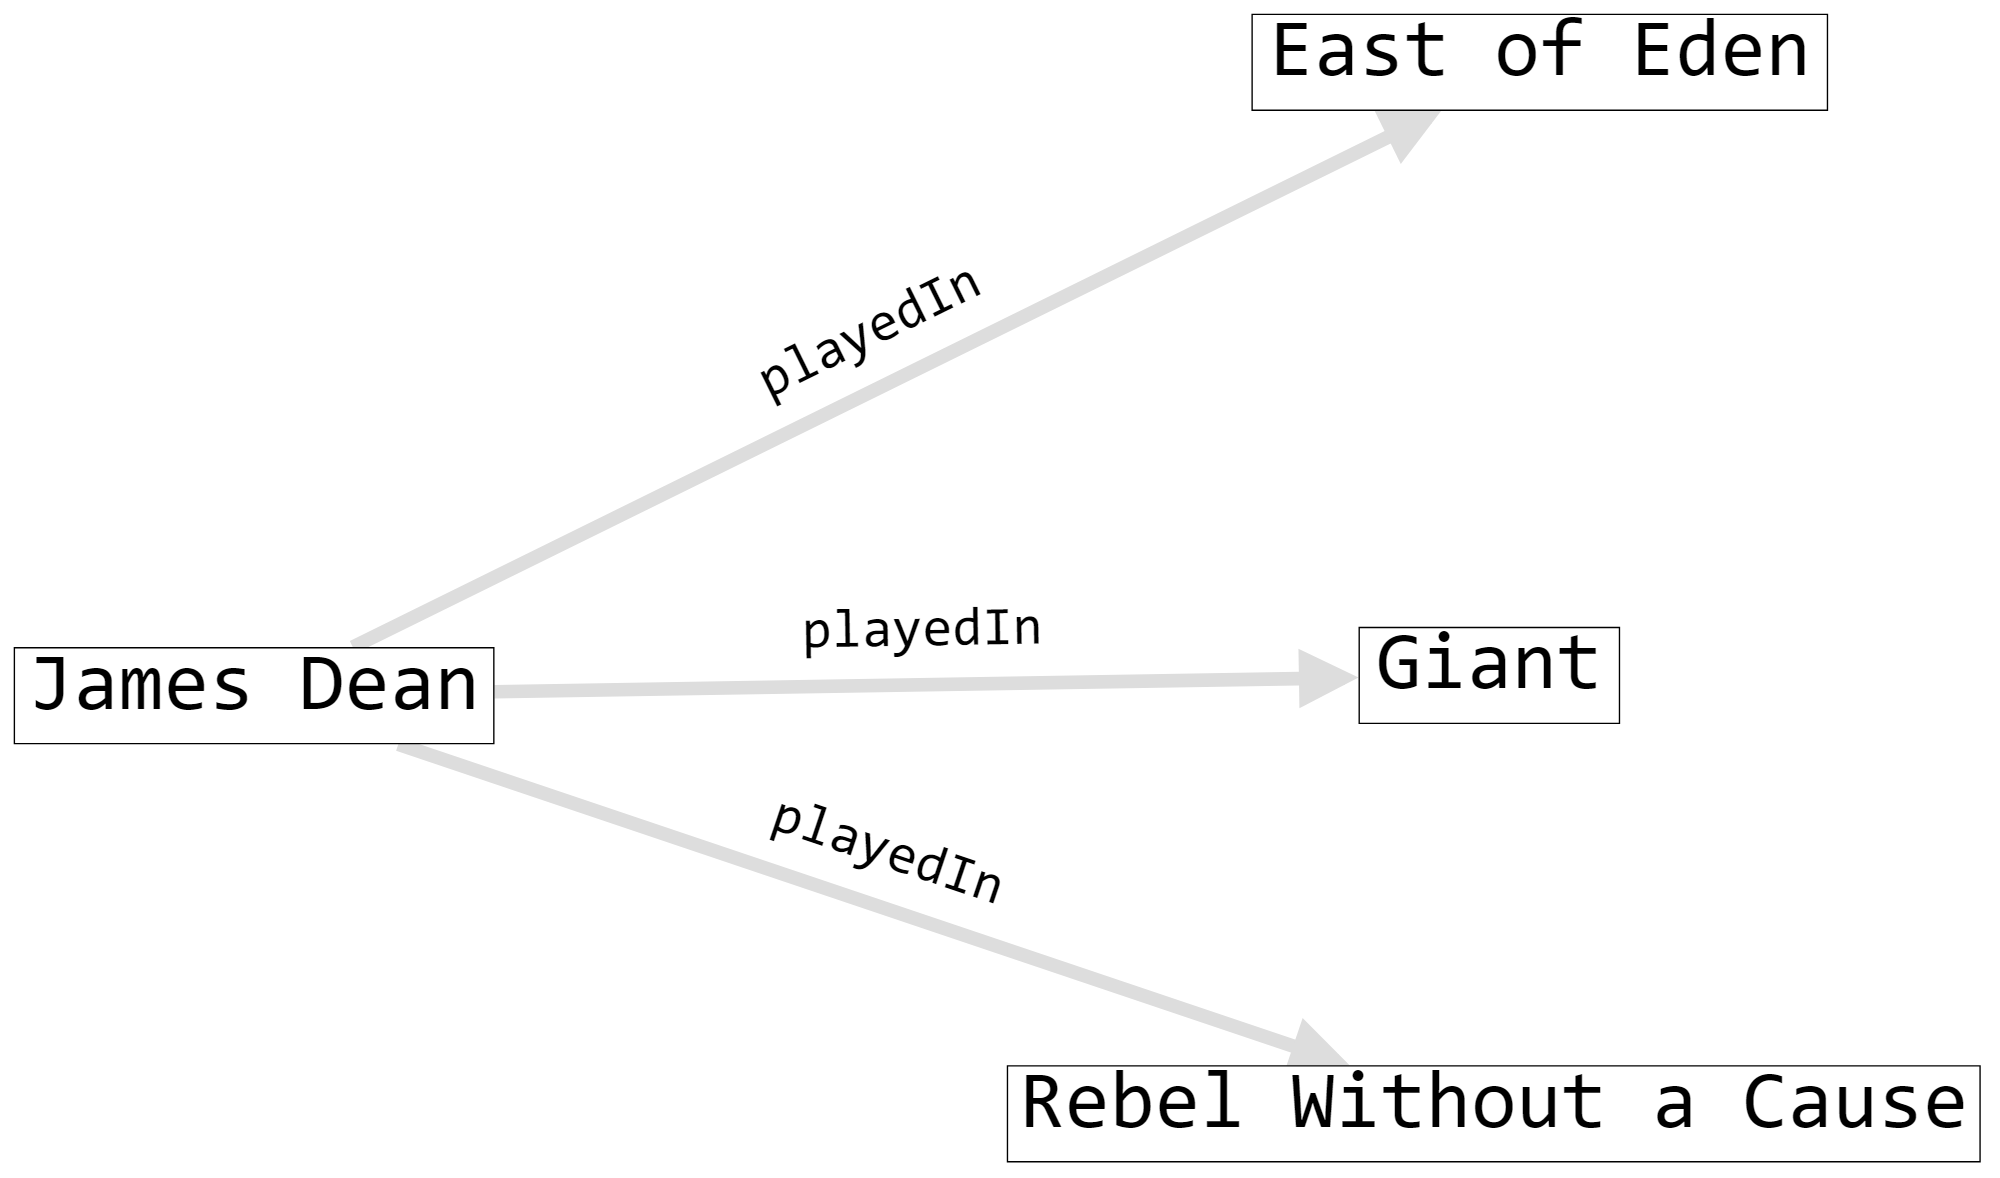
\includegraphics[width=5in]{SWWOv3/media/ch6/figure6-1a.png}
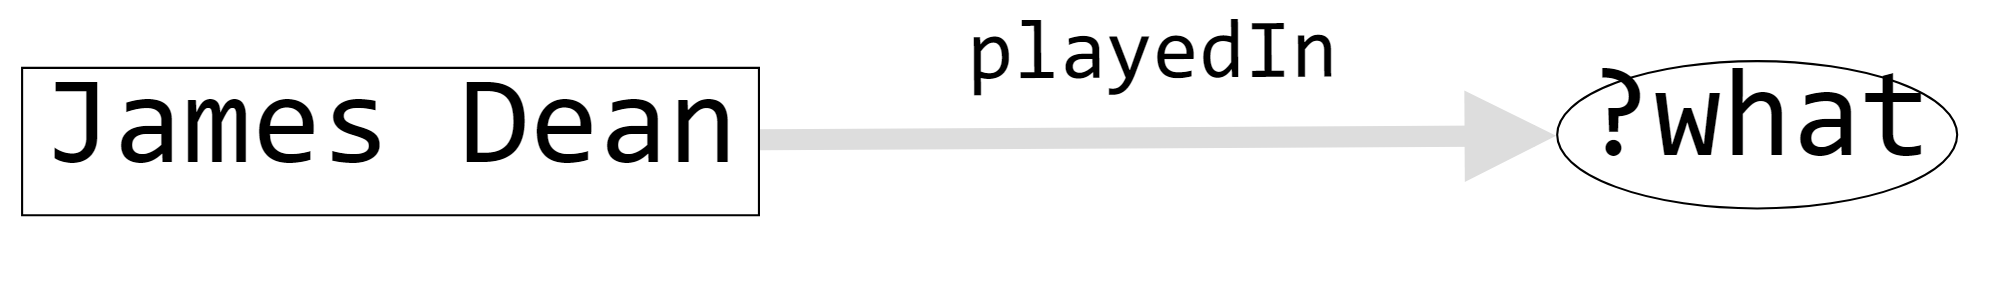
\includegraphics[width=5in]{SWWOv3/media/ch6/figure6-1b.png}
\label{fig:ch06.1}
\caption{James Dean data in a graph, and a query to fetch it.}
\end{figure}

\begin{figure}
\centering
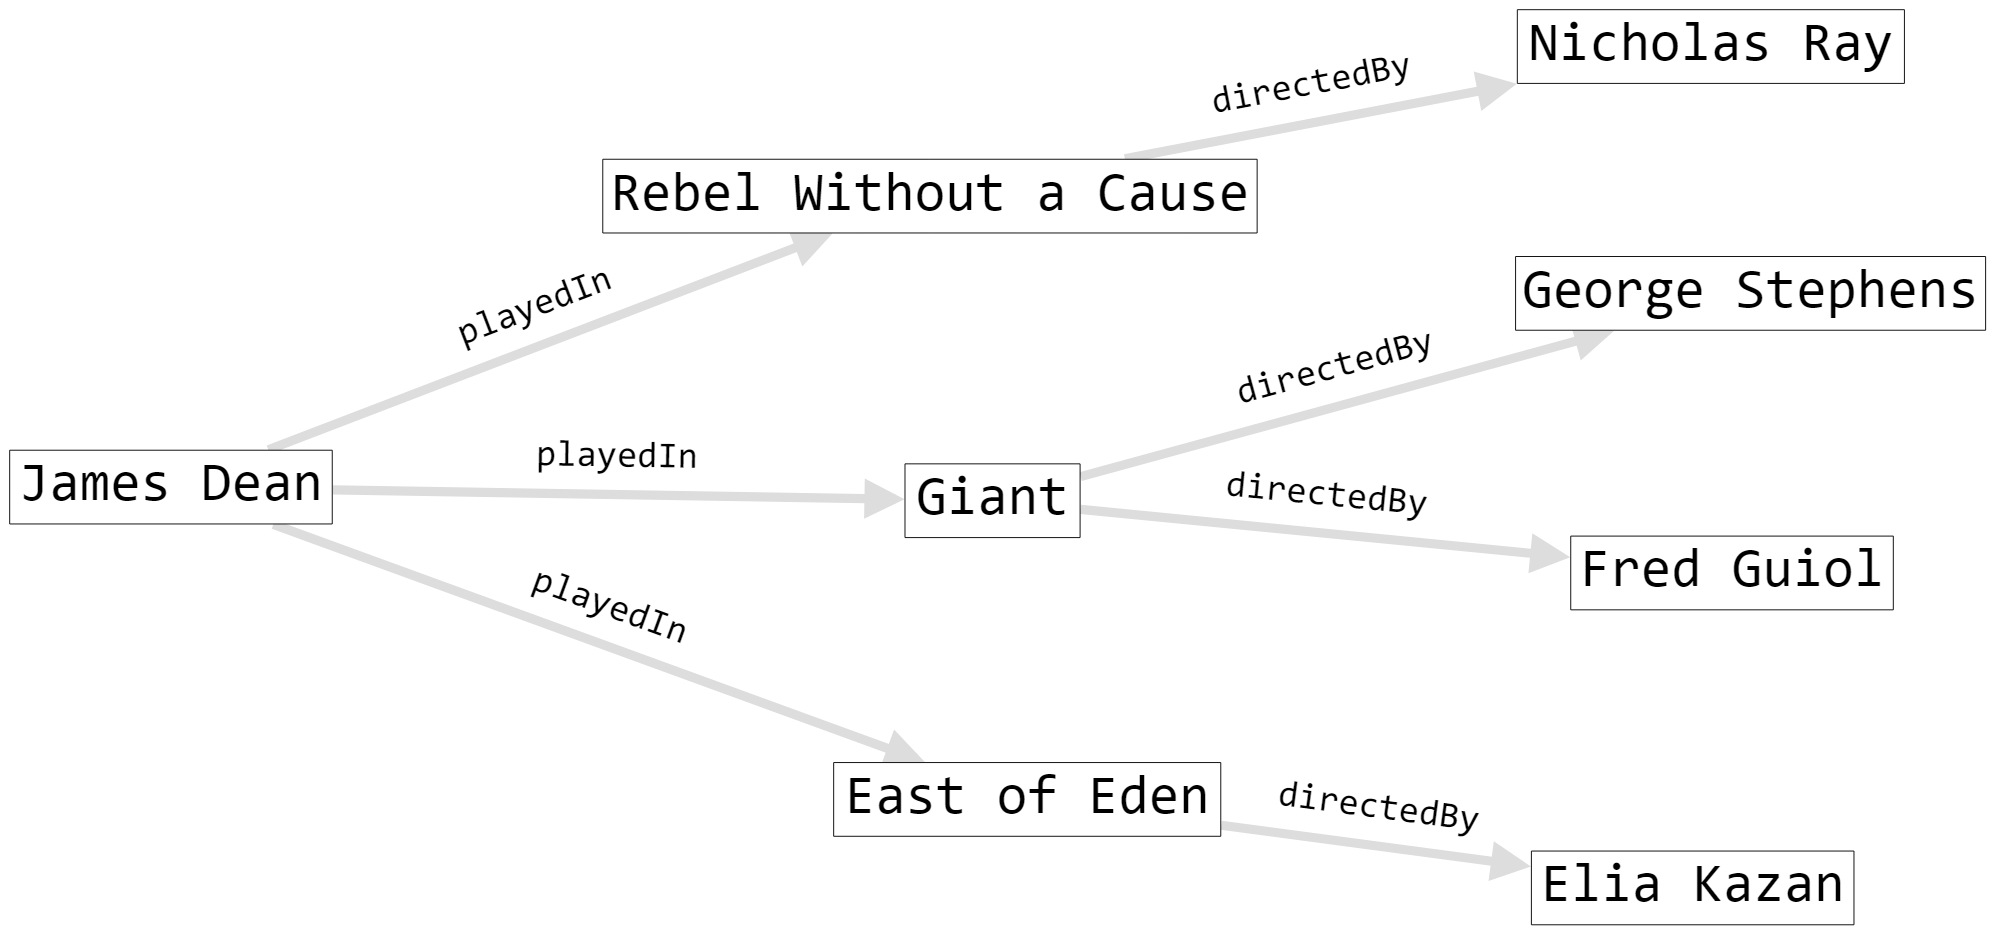
\includegraphics[width=5in]{SWWOv3/media/ch6/figure6-2.png}
\label{fig:ch6.2}
\caption{James Dean's movies and their directors.}
\end{figure}

\begin{figure}
\centering
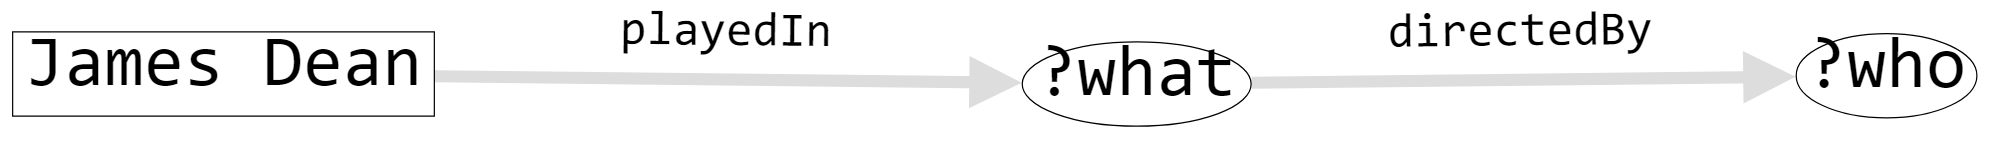
\includegraphics[width=5in]{SWWOv3/media/ch6/figure6-3.png}
\label{fig:ch6.3}
\caption{Graphic version of a query to find James Dean's directors.}
\end{figure}

James Dean worked with? We can query this by asking who directed the
movies that James Dean played in. The graph pattern for this query has
two triples:

\begin{lstlisting}
:JamesDean :playedIn ?what .
?what :directedBy ?who .
\end{lstlisting}

Since the variable \texttt{?what} appears in both triples, the graph pattern is
joined at that point. We can draw a graph pattern the same way we draw a
graph. Figure~\ref{fig:ch6.3} shows this graph pattern. There are two triples in the
pattern and two triples in the diagram.

This graph pattern has two question words, so the query engine will find
all matches for the pattern, with both question words being free to
match any resource. This results in several matches:

\begin{tabular}{ l l }
?what=:Giant&?who=:GeorgeStevens\\
?what=:Giant&?who=:FredGuiol \\
?what=:EastOfEden&?who=:EliaKazan \\
?what=:RebelWithoutaCause&?who=:NicholasRay \\
\end{tabular}

When we have more than one question word, we might actually only be
interested in one of them. In this case, we asked what directors James
Dean had worked with; the movies he played in were just a means to that
end. This is where the details of the SELECT clause come in -- we can
specify which question words we are interested in. So the complete query
to find James Dean's directors looks like this:

\query{Who directed James Dean?}

\begin{lstlisting}
SELECT ?who
WHERE {:JamesDean :playedIn ?what .
       ?what :directedBy ?who . }
\end{lstlisting}

\textbf{\textbf{Answer:}}

\begin{lstlisting}
:GeorgeStevens, :EliaKazan, :NicholasRay, :FredGuiol
\end{lstlisting}

Since a query in SPARQL can have several question words and several
answers, it is convenient to display the answers in a table with one
column for each question word and one row for each answer.

\begin{tabular}{|l|}
\hline
?who\\
\hline
:GeorgeStevens\\
:EliaKazan\\
:NicholasRay\\
:FredGuiol\\
\hline
\end{tabular}

If we decide to keep both question words in the SELECT, we will have
more columns in the table

\query{Why directed James Dean movies?}

\begin{lstlisting}
SELECT ?what ?who
WHERE {:JamesDean :playedIn ?what .
       ?what :directedBy ?who .}
\end{lstlisting}

\begin{tabular}{| l l | }
\hline
?what&?who\\
\hline
:Giant&:GeorgeStevens\\
:Giant&:FredGuiol\\
:EastOfEden&:EliaKazan\\
:RebelWithoutaCause&:NicholasRay\\
\hline
\end{tabular}

\subsection{Naming question words in SPARQL}

In English, we have a handful of question words -- who, what, where,
etc. A question doesn't make sense if we use some other word. But in
SPARQL, a question word is just signaled by the ? at the start -- any
word would do just as well. If we look at the output table above, the
question words \texttt{?who} and \texttt{?what} are not very helpful in describing what is
going on in the table. If we remember the question, we know what they
mean (\texttt{?what} is a movie, and \texttt{?who} is its director). But we can make the
table more understandable, even out of the context of the question, by
selecting descriptive question words. It is customary in SPARQL to do
this, to communicate the intention of a question word to someone who
might want to read the query. For example, we might write this query as

\textbf{\textbf{Ask:}}

\begin{lstlisting}
SELECT ?movie ?director
WHERE {:JamesDean :playedIn ?movie .
       ?movie :directedBy ?director .}
\end{lstlisting}

\textbf{\textbf{Answer:}}

\begin{tabular}{|ll|}
\hline
?movie&?director\\
\hline
:Giant&:GeorgeStevens\\
:Giant&:FredGuiol\\
:EastOfEden&:EliaKazan\\
:RebelWithoutaCause&:NicholasRay\\
\hline
\end{tabular}

The graph pattern we just saw was a simple chain -- James Dean played in
some movie that was directed by someone. Graph patterns in SPARQL can be
as elaborate as the graphs they match against. For instance, given a
more complete set of information about James Dean movies we could find
the actresses who worked with him with a graph pattern:

\query{Actresses who worked with James Dean}

\begin{lstlisting}
SELECT ?actress ?movie
WHERE {:JamesDean :playedIn ?movie .
       ?actress :playedIn ?movie .
       ?actress rdf:type :Woman }
\end{lstlisting}

\textbf{\textbf{Answer:}}

\begin{tabular}{|l|}
\hline
?actress\\
\hline
:AnnDoran\\
:ElizabethTaylor\\
:CarrollBaker\\
:JoVanFleet\\
:JulieHarris\\
:MercedesMcCambridge\\
:NatalieWood\\
\hline
\end{tabular}

Figure~\ref{fig:ch6.4} shows a fragment of the data graph, and the graph pattern,
with the result for the question word \texttt{?actress} indicated in the third
`column' of the figure. Notice that Rock Hudson is not a match; while he
indeed played in \emph{Giant}, there is no match for the third triple,

\begin{lstlisting}
:RockHudson rdf:type :Woman.
\end{lstlisting}

\begin{figure}
\centering
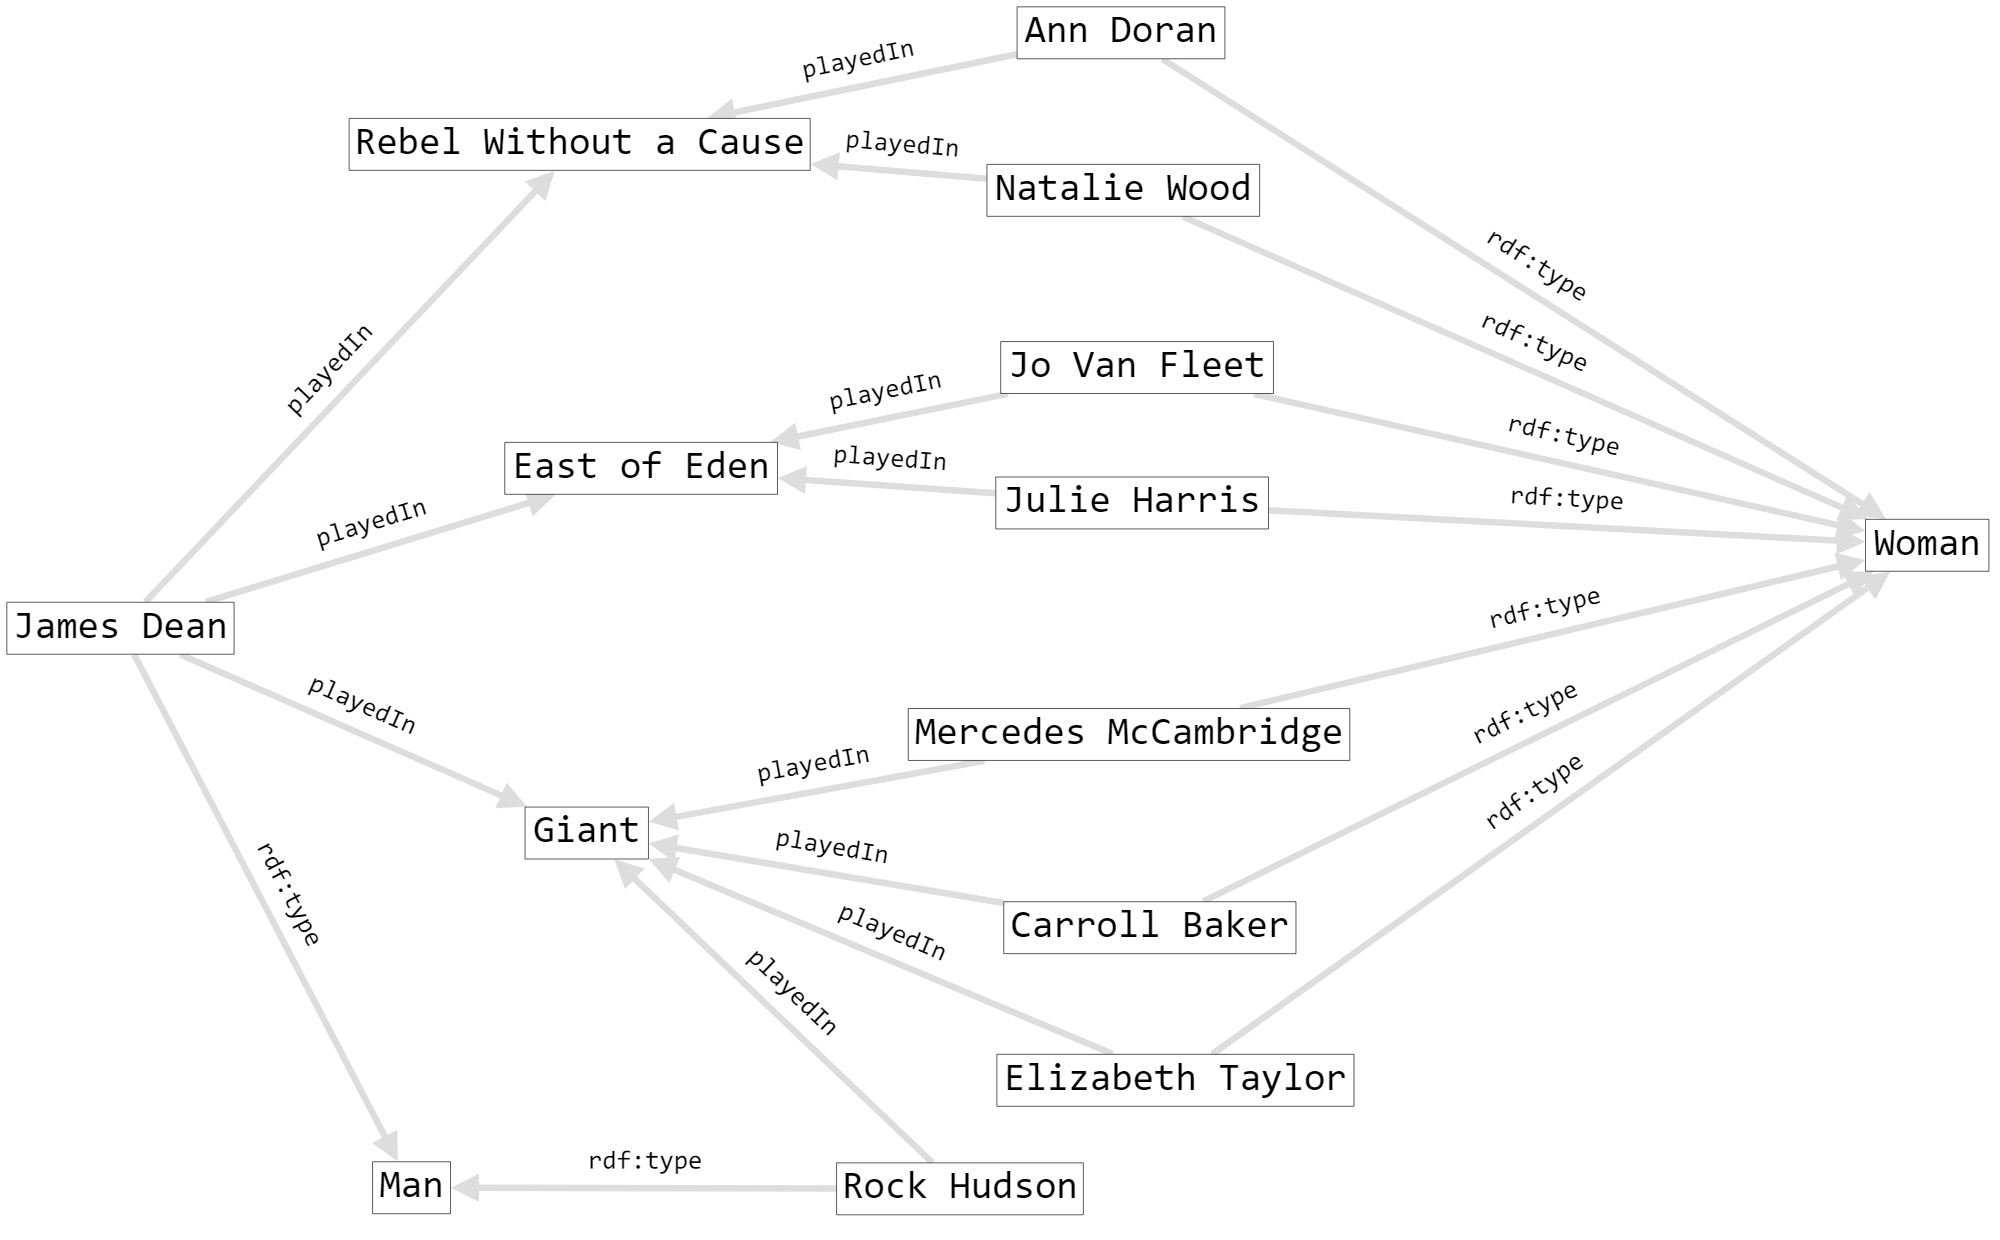
\includegraphics[width=5in]{SWWOv3/media/ch6/figure6-4a.png}
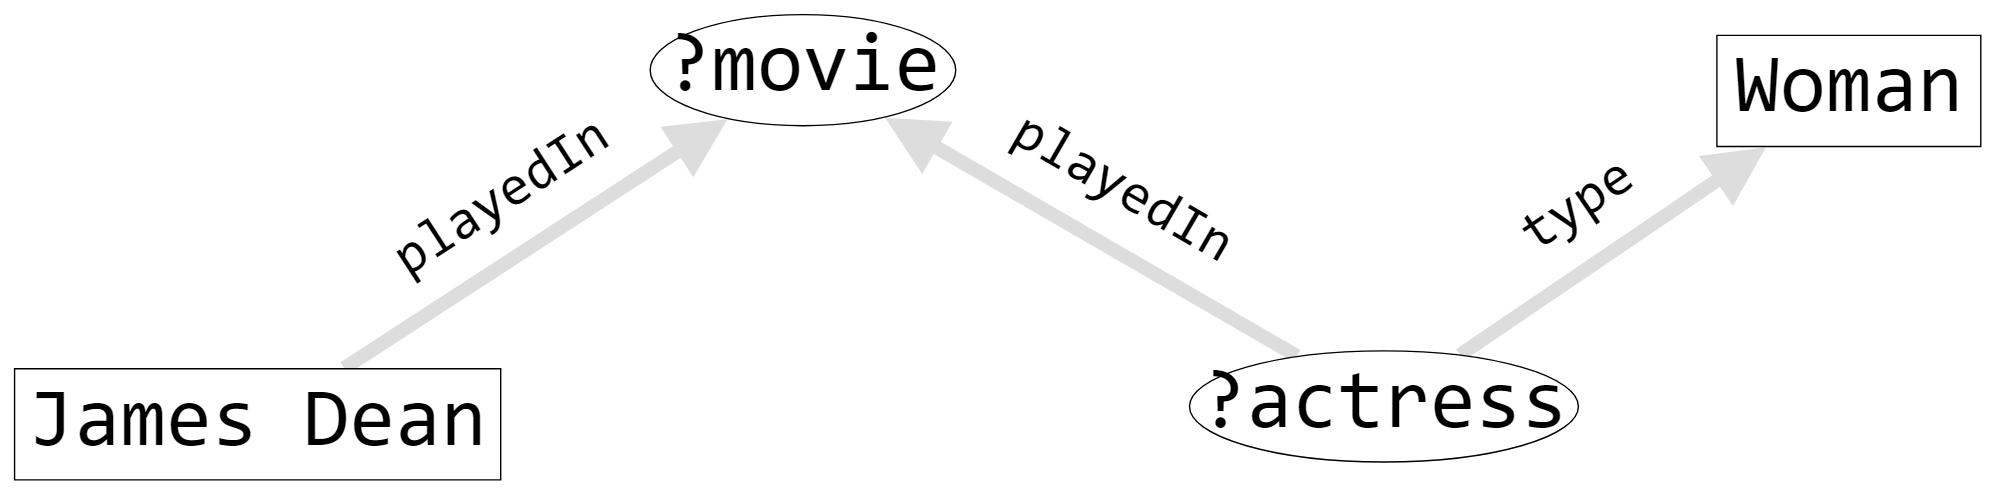
\includegraphics[width=5in]{SWWOv3/media/ch6/figure6-4b.png}
\label{fig:ch6.4}
\caption{Information about James Dean's co-stars, and a query to fetch some of it.}
\end{figure}

Remember that \texttt{?actress} is just a question word like \texttt{?who}, renamed to be
more readable; the only reason \texttt{?actress} doesn't match \texttt{:RockHudson} is
because the data do not support the match. That is, the meaning of
\texttt{?actress} is not given by its name, but instead by the structure of the
graph pattern.

With this observation, one might wonder how we know that \texttt{?movie} is sure
to come up with movies? And indeed, this is a consideration; in this
example, the only things that James Dean played in were movies, so it
really isn't an issue. But on the Semantic Web, we could have more
information about things that James Dean played in. So we really should
restrict the value of the question word \texttt{?movie} to be a member of the
class movie. We can do this by adding one more triple to the pattern:

\query{Movie actresses who worked with James Dean}

\begin{lstlisting}
SELECT ?actress
WHERE {:JamesDean :playedIn ?movie .
       ?movie rdf:type :Movie .
       ?actress :playedIn ?movie .
       ?actress rdf:type :Woman  }
\end{lstlisting}

This query pattern is shown graphically in Figure\ref{fig:ch6.5}. Triples like

\begin{lstlisting}
?movie rdf:type :Movie .
\end{lstlisting}

can seem a bit confusing at first -- with two uses of the word movie,
what does this mean? But now that we know that \texttt{?movie} is just a generic
question word with a name that prints well in a table, we can see that
this triple is how we tell SPARQL what we really mean by \texttt{?movie}. The
meaning isn't in the name, so we have to put it in a triple.

You might come upon a model that gives properties the same name as the
class of entity they are intended to point to -- so that instead of a
property called \texttt{:directedBy} in this example, a model might call it
simply \texttt{:director}. In such a case, the query to find the people who
directed James Dean movies would look like this:

\query{Who was director for James Dean?}
\begin{lstlisting}
SELECT ?director
WHERE {:JamesDean :playedIn ?movie .
       ?movie :director ?director .}
\end{lstlisting}

\begin{figure}
\centering
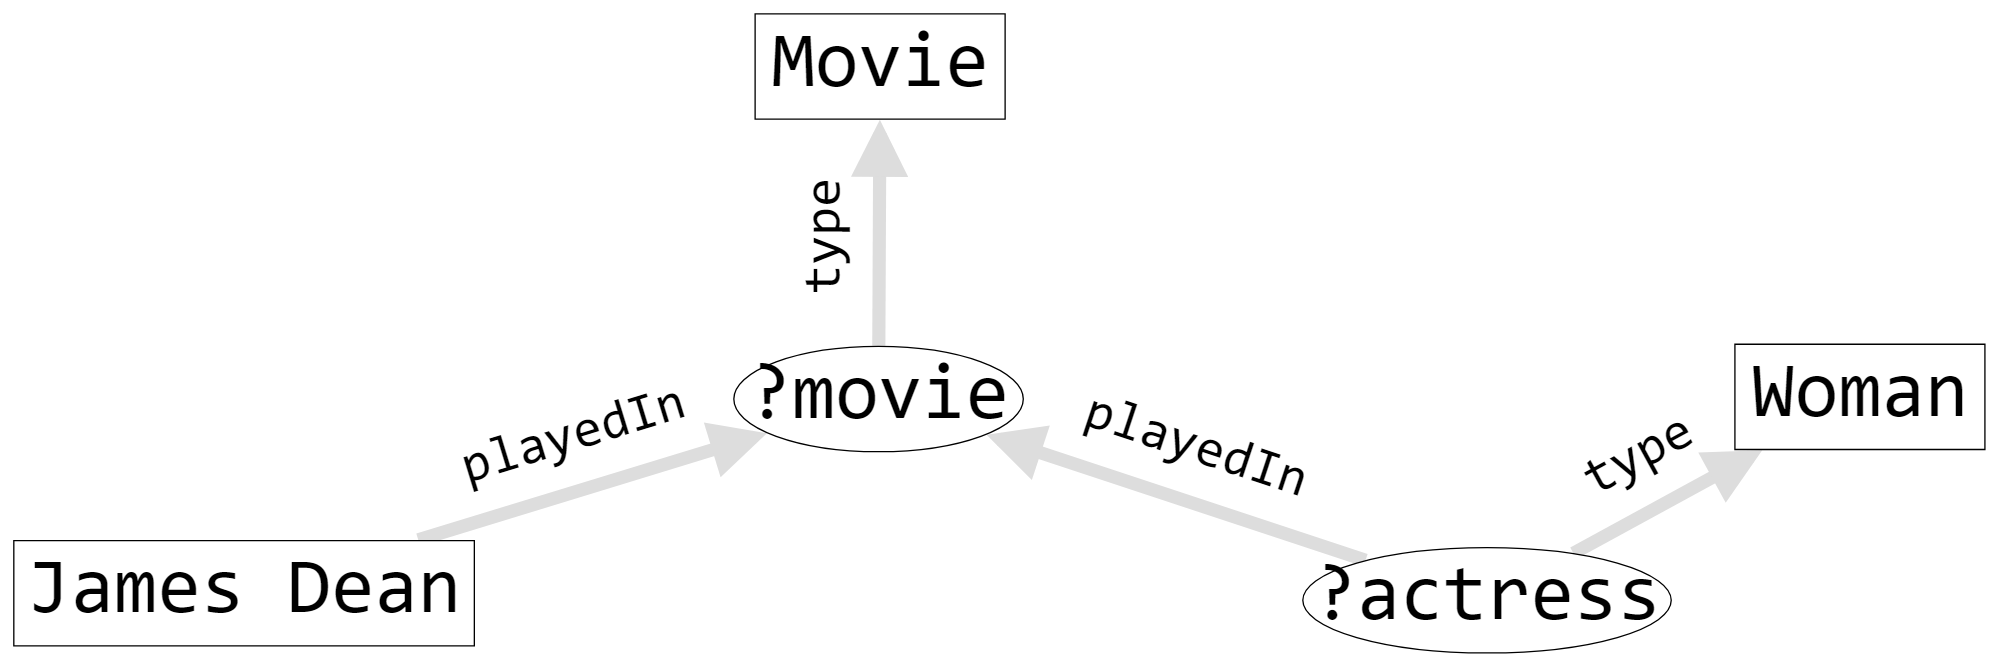
\includegraphics[width=5in]{SWWOv3/media/ch6/figure6-5.png}
\label{fig:ch6.5}
\caption{Extended query pattern that includes the fact that ?movie has type Movie.
}
\end{figure}

This can look a bit daunting -- what is the difference between \texttt{?director}
and \texttt{:director}? As we've already seen, \texttt{:director} refers to a particular
resource (using the default namespace -- that's what the ``:'' means) On
the other hand, \texttt{?director} is a question word -- it could have been \texttt{?foo}
or \texttt{?bar} just as easily, but we chose \texttt{?director} to remind us of its
connection with a movie director, when we see it out of the context of
the query. If you have to write (or read!) a query written for a model
that names its properties in this way, don't panic! Just remember that
the ? marks a question word -- the name \texttt{?director} is just there to let
you (and whoever else reads the query) know what \texttt{?director} is expected
to mean. If you are creating your own model, we recommend that you use
property names like \texttt{:directedBy} instead of \texttt{:director} so that you don't
invite this confusion in the people who want to query data using your
model.

\subsection{Query structure vs. data structure}

In Figure~\ref{fig:ch6.4}, we saw how the graph pattern in a query looks a lot like
the data graph it matches against. This is true of graph patterns in
general. The complexity of a question that can be specified with SPARQL
is limited only by the complexity of the data. We could, for instance,
ask about actresses who played in a movie with James Dean who themselves
were in a movie directed by John Ford:

\query{James Dean co-stars directed by John Ford}
\begin{lstlisting}
SELECT ?actress ?movie
WHERE {:JamesDean :playedIn ?movie .
       ?actress :playedIn ?movie .
       ?actress a :Woman .
       ?actress :playedIn ?anotherMovie .
       ?anotherMovie :directedBy :JohnFord .}
\end{lstlisting}

\textbf{\textbf{Answer:}}

\begin{tabular}{|l|}
\hline
?actress\\
\hline
NatalieWood\\
CarrollBaker\\
\hline
\end{tabular}

Figure~\ref{fig:ch6.6} shows this query as a graph. In the text version of the
query, we often see the same question word appear in multiple triples,
and some of them even refer to the same kind of thing (\texttt{?movie},
\texttt{?anotherMovie}). In the graph version, we see that these are the points
where two triples must refer to the same thing. For instance, we know
that James Dean and \texttt{?actress} played in the same movie, because both
triples use the same question word (\texttt{?movie}) for that movie. Similarly,
that \texttt{?actress} is the same one who played in \texttt{?anotherMovie}, because there
the same question word \texttt{?actress} appears in those two triples. All these
relationships are visibly apparent in Figure\ref{fig:ch6.6}, where we see that
\texttt{?movie} is the connection between James Dean and \texttt{?actress}, \texttt{?actress} is
the connection between \texttt{?movie} and \texttt{?anotherMovie}, and \texttt{?anotherMovie} is
the connection between \texttt{?actress} and John Ford.

If we look at the information supporting the answer ``Natalie Wood,'' we
see that the data graph looks just like the graph pattern -- this should
come as no surprise, since that is how the pattern works. But we can use
this feature to our advantage when writing queries. One way to write a
complex query like the one in Figure\ref{fig:ch6.6} is to walk through the question
we want to answer, writing down triples as we go until we have the full query. But another way is to start with the
data. Suppose we have an example of what we want to search for, for
example, we know that Natalie Wood played in The Searchers, which was
directed by John Ford. Next, we show how we can use the close match
between graphs and patterns to construct the pattern from the example.


\begin{figure}
\centering
(a)
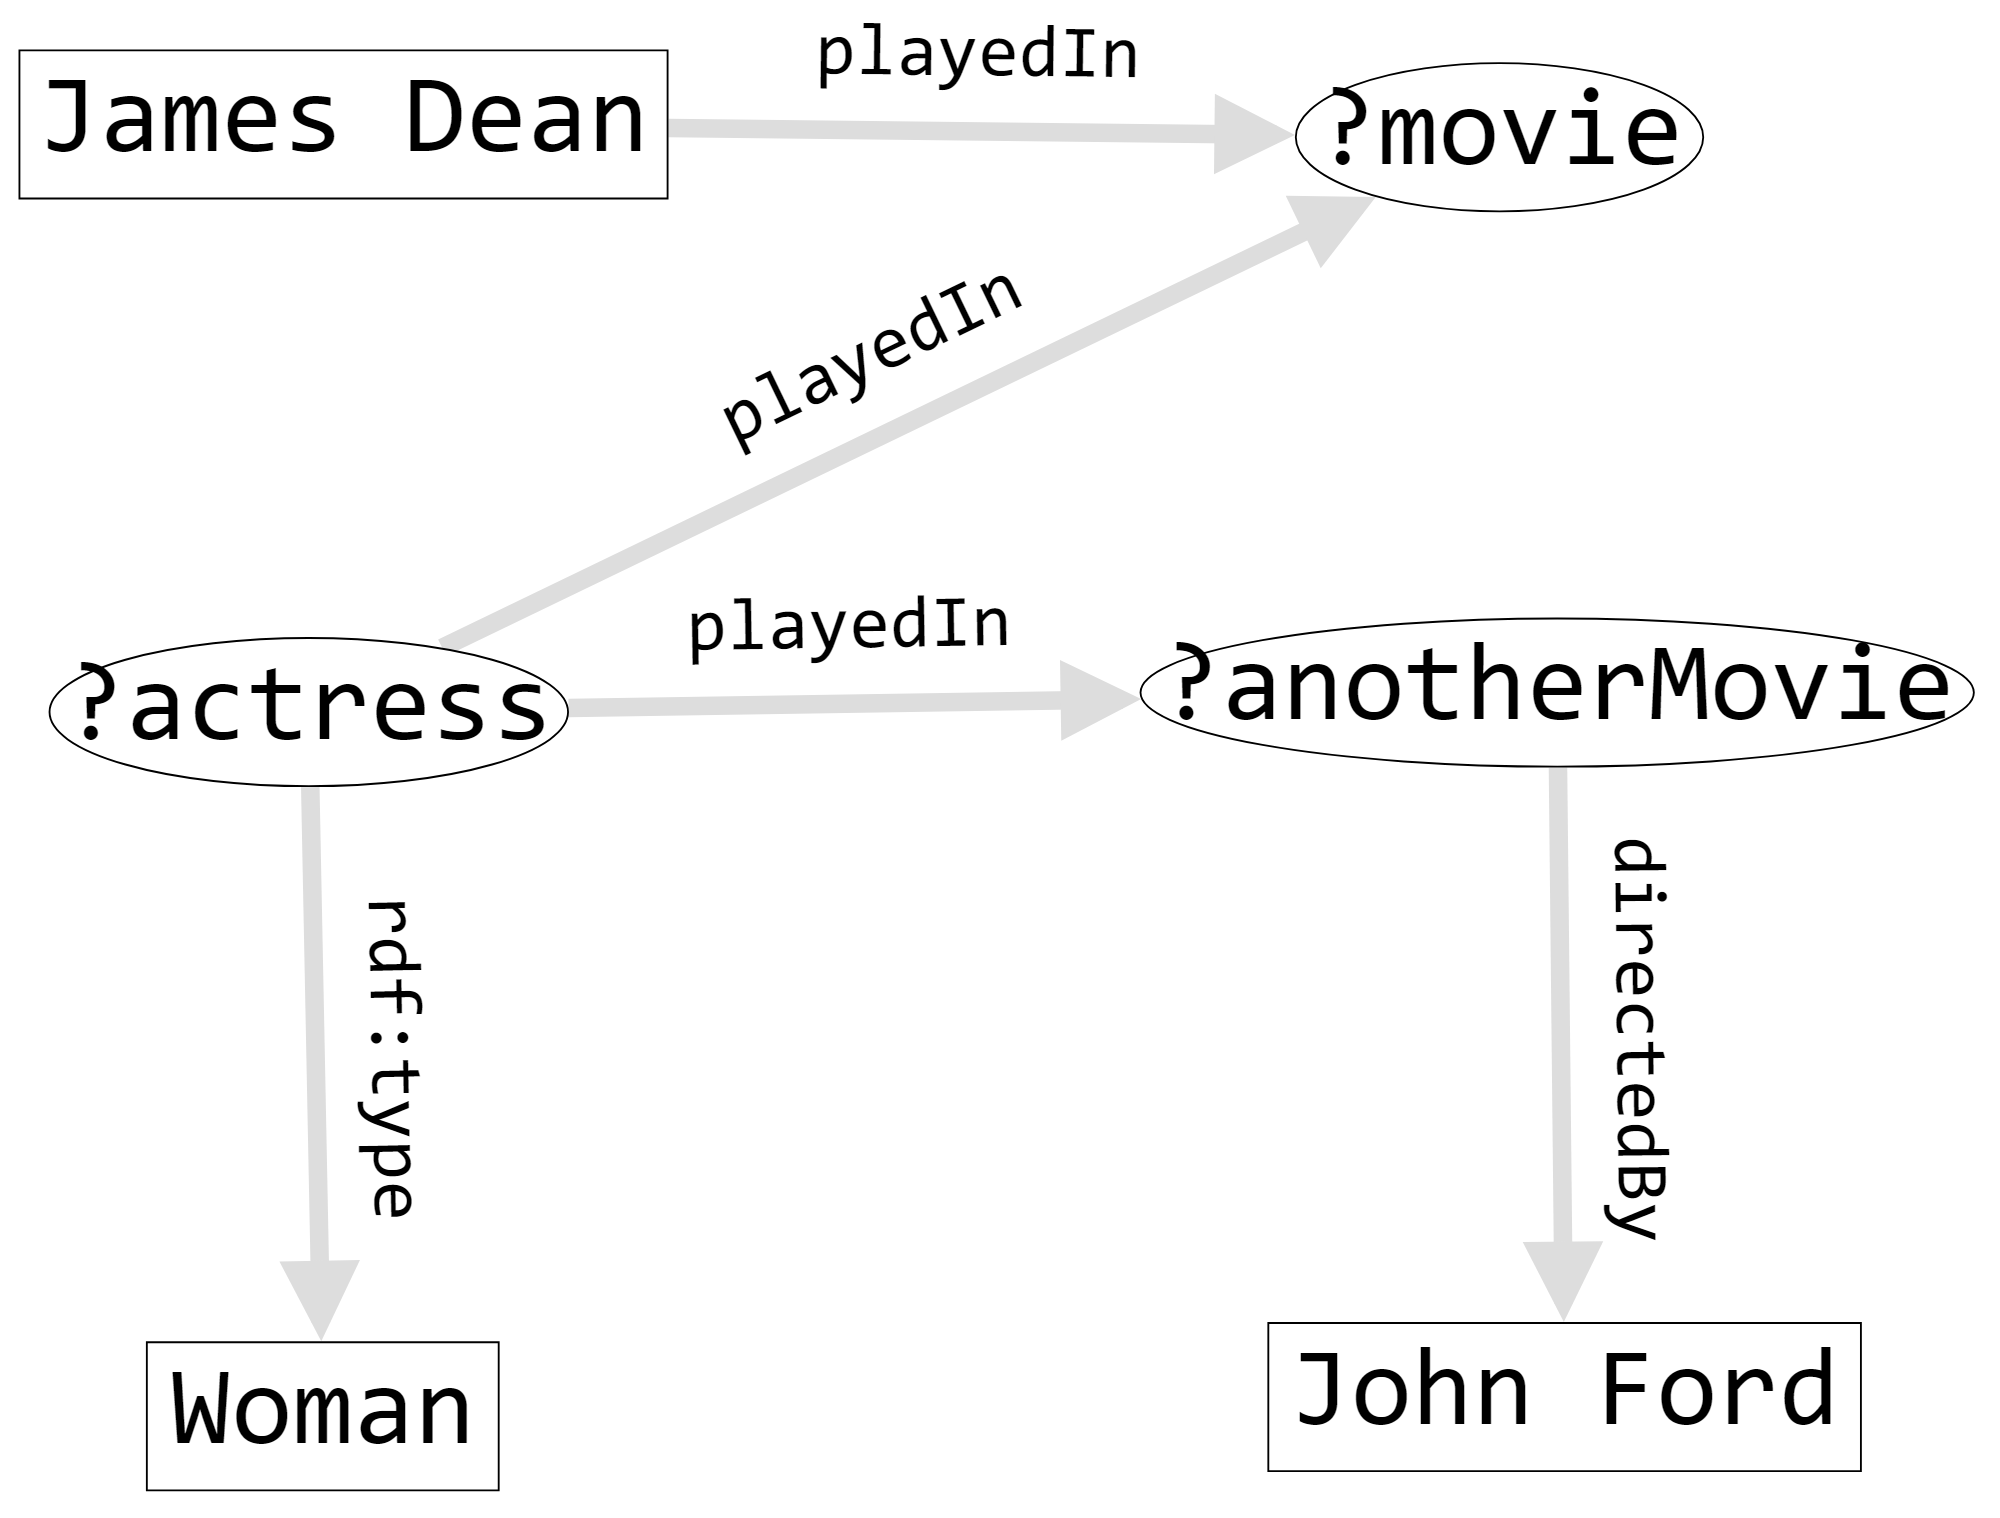
\includegraphics[width=5in]{SWWOv3/media/ch6/figure6-6a.png}
(b)
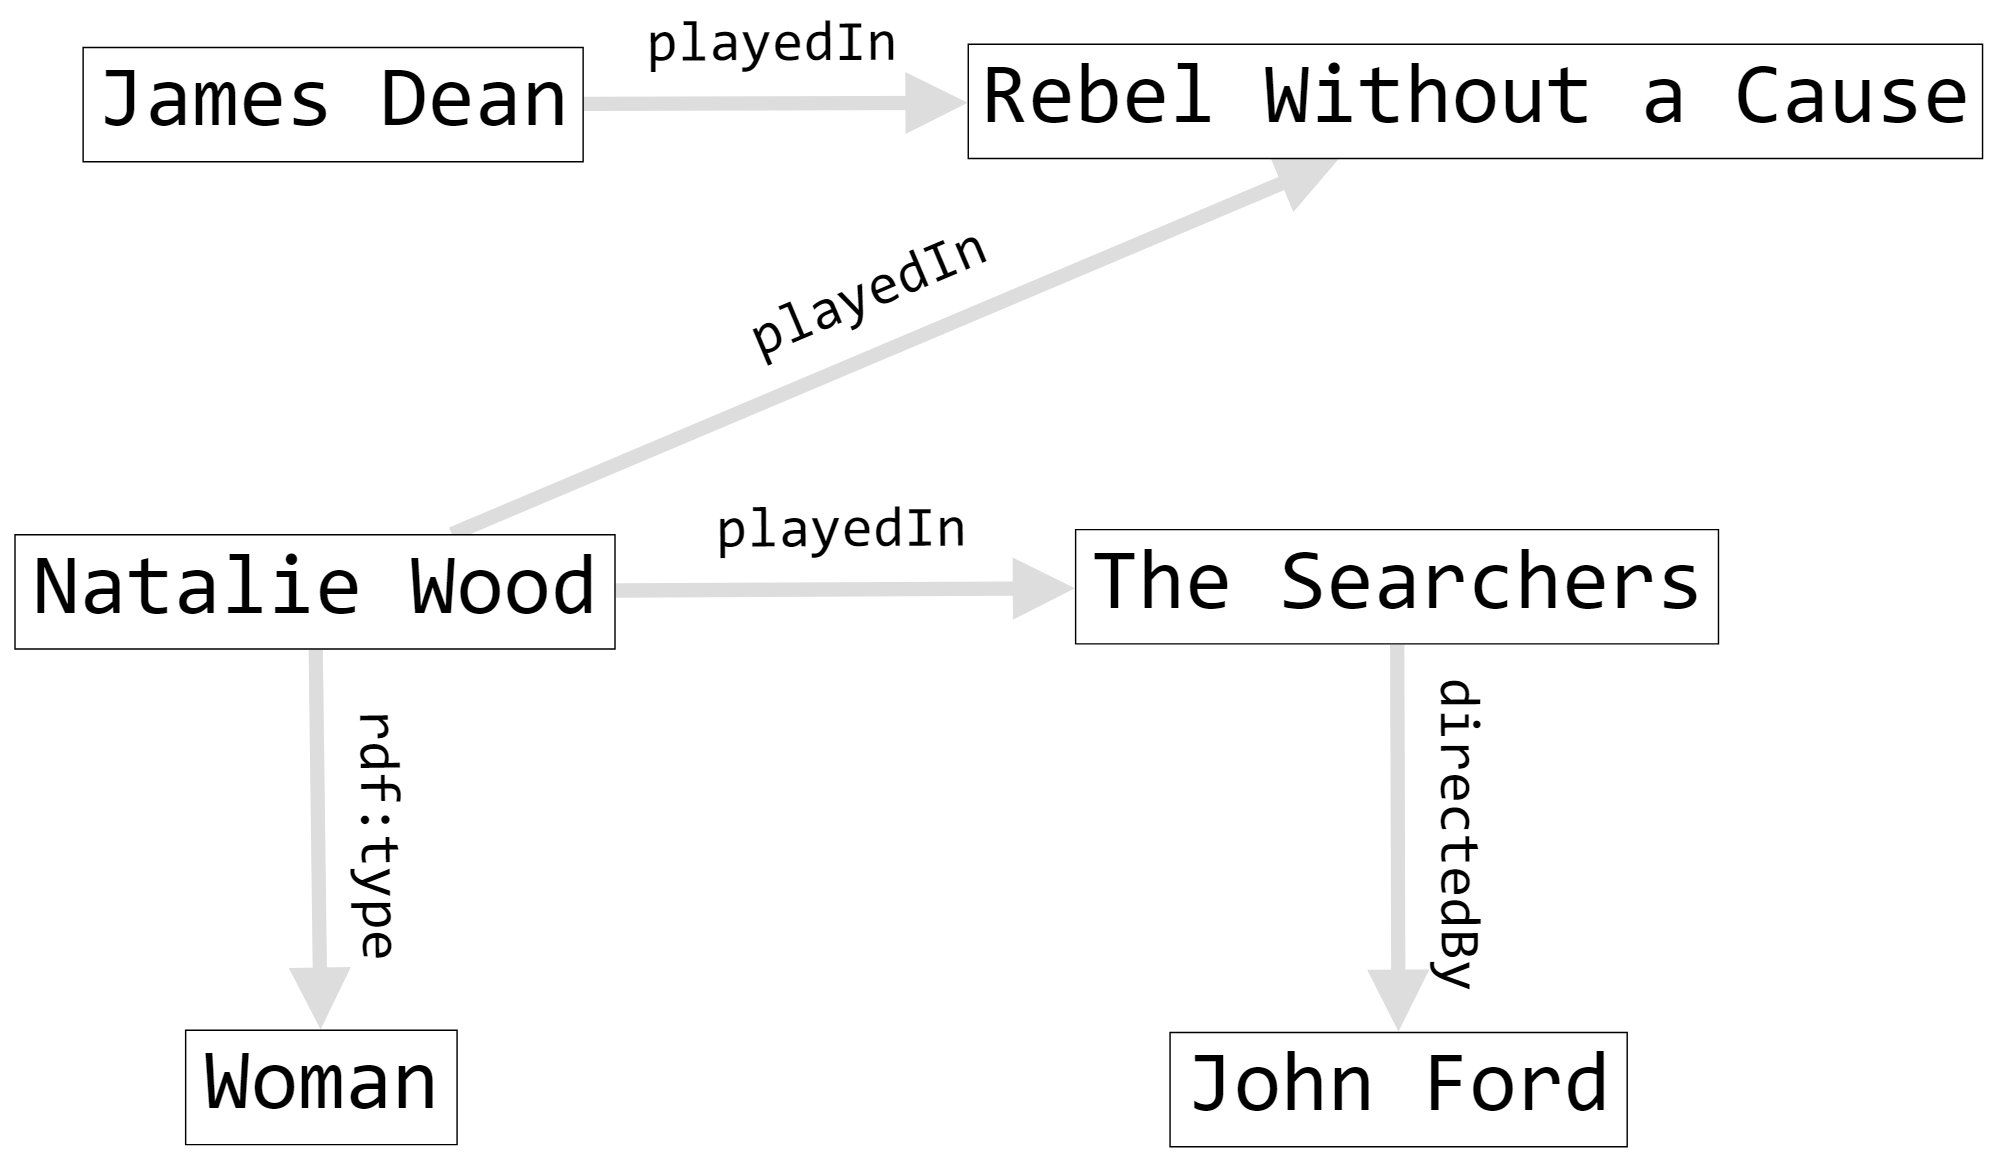
\includegraphics[width=5in]{SWWOv3/media/ch6/figure6-6b.png}
\label{fig:ch6.6}
\caption{Data about James Dean and Natalie Wood, and a query to fetch that data.}
\end{figure}


Since the example from the data graph matches the graph pattern triple
for triple, we already know a lot about the graph pattern we want to
create. The only thing we need to specify is which values from the
example we want to keep as literal values in the pattern, and which ones
we want to replace with
question words. In Figure\ref{fig:ch6.7}(a) the boxed x on certain resources (James
Dean, John Ford, and Woman) indicates those that will stay as they are;
all other resources (Natalie Wood, The Searchers, \emph{Rebel without a
Cause}) will be replaced with question words. We have to decide what
question words to use; there could be a lot of them. Remember that as
far as the SPARQL query engine is concerned, the names of the question
words aren't important, so we can call them whatever we like as long as
we make sure to use the same question word when we need the same value
to be used in the answer. For this example, we'll call them \texttt{?q1}, \texttt{?q2},
etc. Figure\ref{fig:ch6.7}(b) shows the query pattern graphically.

\begin{figure}
\centering
(a)
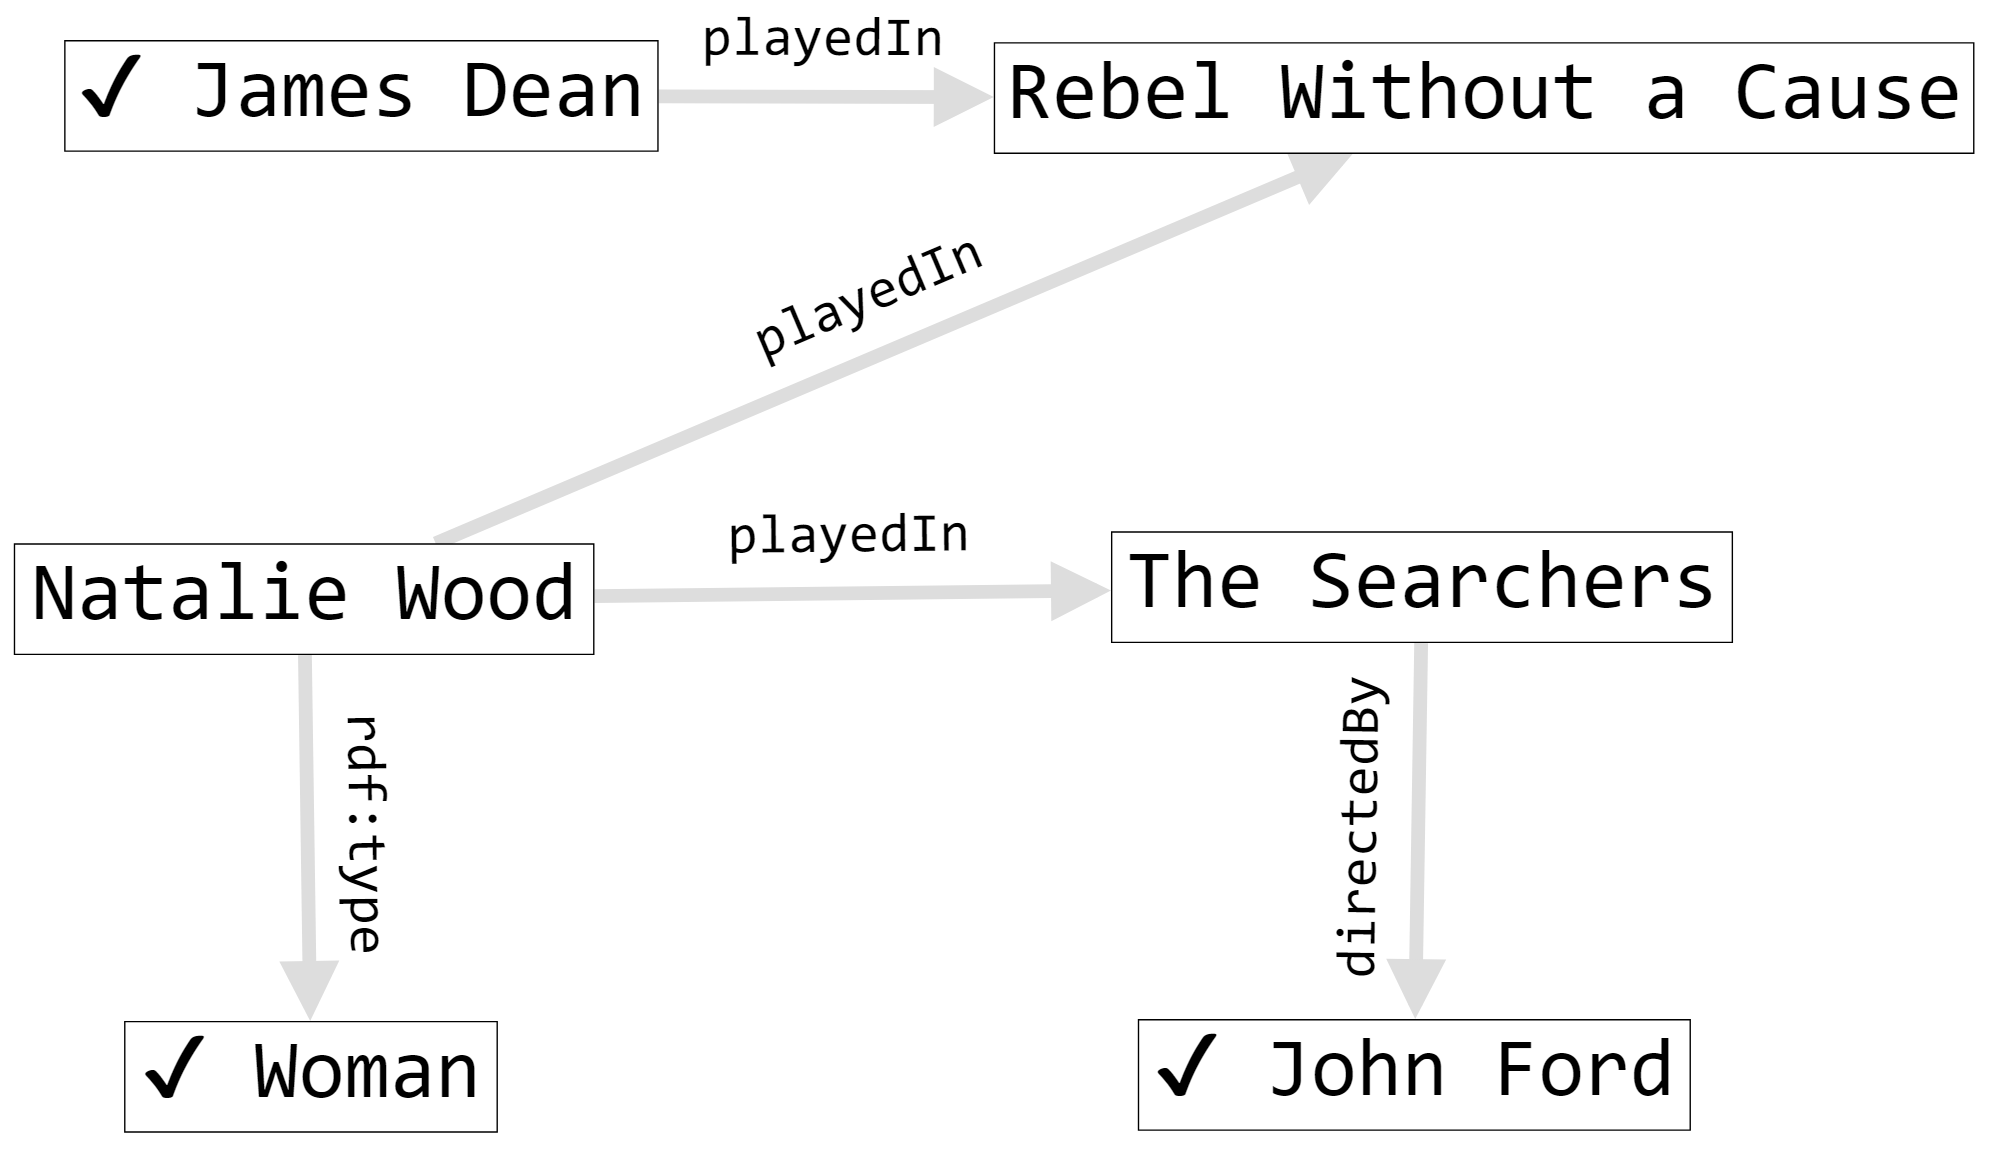
\includegraphics[width=5in]{SWWOv3/media/ch6/figure6-7a.png}
(b)
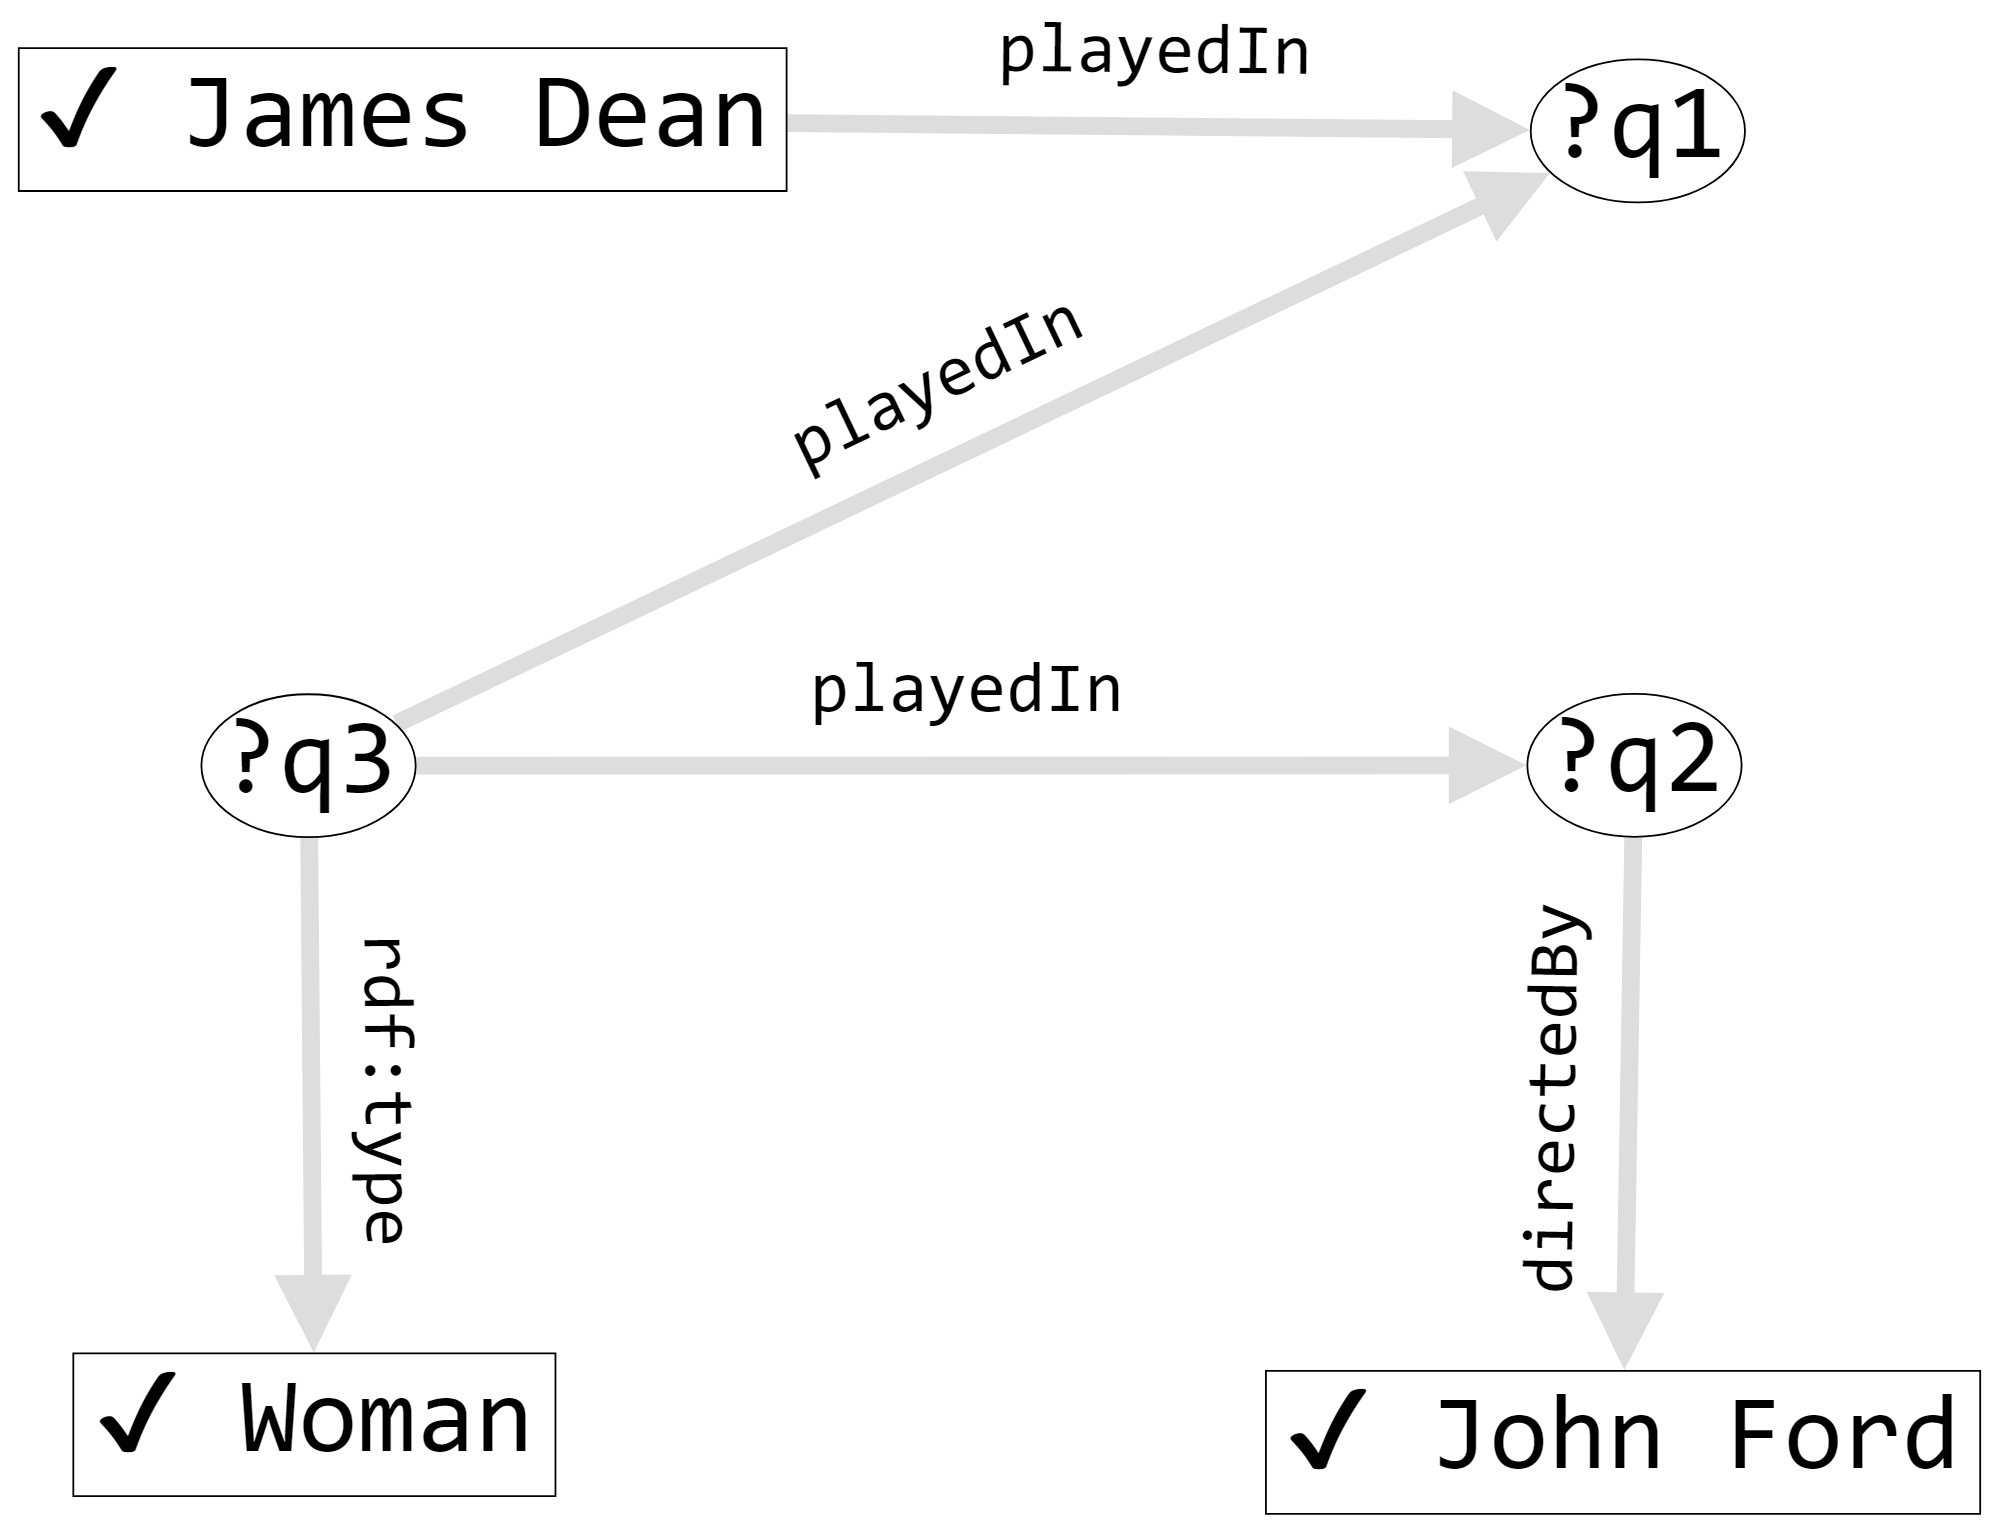
\includegraphics[width=5in]{SWWOv3/media/ch6/figure6-7b.png}
\label{fig:ch6.7}
\caption{Creating a graph pattern from a data graph. Resources marked with X appear as themselves in the query.}
\end{figure}


Now we can create our SPARQL query by simply copying down the graph
pattern in Turtle. Each arrow in the graph becomes a triple. If a
particular entity (either a literal resource or a question word)
participates in more than one triple in the graph, then it will appear
more than one time in the Turtle rendering of the pattern. The graph
diagram in Figure\ref{fig:ch6.7}(b) has five connecting arrows; the corresponding
query will have the same number of triples:

\begin{lstlisting}
{ :JamesDean :playedIn ?q1 .
   ?q3 :playedIn ?q1 .
   ?q3 rdf:type :Woman .
   ?q3 :playedIn ?q2 .
   ?q2 :directedBy :JohnFord .}
\end{lstlisting}

To complete the query, simply SELECT the question word(s) you want to
report on, and perhaps give it a meaningful name. This brings us back to
a query very like the original query (differing only in the names of the
unselected question words) -- but this time, it was generated from a
pattern in the data.

\query{Generated query for Women who worked with James Dean and John Ford}
\begin{lstlisting}
SELECT ?actress
WHERE {:JamesDean :playedIn ?q1 .
       ?actress :playedIn ?q1 .
       ?actress rdf:type :Woman .
       ?actress :playedIn ?q2 .
       ?q2 :directedBy :JohnFord . }
\end{lstlisting}


As we saw above, there are two matches for this query in the sample
data, Natalie Wood (no surprise there -- after all, it was her
performance that we used as a model for this query) and Carroll Baker.
Carroll Baker is similar to Natalie Wood, in that she is also a woman,
she also played alongside James Dean in a movie, and she was also
directed by John Ford. She is similar to Natalie Wood in exactly the
features specified in the query.

This method for creating queries can be seen as a sort of ``more like
this'' capability; once you have one example of something you are
interested in, you can ask for ``more like this,'' where the notion of
``like this'' is made specific by including particular triples in the
example, and hence in the graph pattern.

For example, we just wrote a query that found actresses who played in
James Dean movies and also played in movies directed by John Ford. How
do we know that the results are limited to actresses? In the example,
Natalie Wood is an actress. But she is one of the resources that we
replaced by a question word -- how do we know that all the things that
the pattern matches will also be actresses? We know this because we
included the triple

\begin{lstlisting}
?q3 rdf:type :Woman .
\end{lstlisting}

in the example, and hence in the pattern.

What would happen if we left that triple out? Natalie Wood is, of
course, still a Woman in the data graph, but we haven't included that
fact in our example. So that fact does not get copied into the query.
Our new query looks like this:

\query{Actors who worked with James Dean and John Ford}
\begin{lstlisting}
SELECT ?q3
WHERE { :JamesDean :playedIn ?q1 .
        ?q3 :playedIn ?q1 .
        ?q3 :playedIn ?q2 .
        ?q2 :directedBy :JohnFord . }
\end{lstlisting}

It has one fewer triple than the previous query. What is the difference
if we run this query against the data? Now we get another answer --
Raymond Massey (who also played in \emph{East of Eden}). It would be
misleading (but perfectly fine from the point of view of the SPARQL
query language) to name this question word \texttt{?actress} in this situation --
we might want to call it \texttt{?actor} instead (with the convention that women
can also be actors; if we don't like that convention, we might just keep
the meaningless name \texttt{?q3}).

So when we say we want to match ``more like this'' from the example of
Natalie Wood, in the first case, we meant ``Women who played with James
Dean in some movie, and who played in a movie directed by John Ford.''
In the second case, we just asked for ``Anyone (even anything) who
played with James Dean in some movie, and who played in a movie directed
by John Ford.'' How did we specify the difference? By including (or
excluding) the triple that asserts that Natalie Wood is a woman. When we
include it, ``more like this'' includes the fact that the result must be
a Woman. When we exclude it, ``more like this'' does not include this
stipulation.

\subsection{Ordering of triples in SPARQL queries}

In the previous section, we copied down a graph pattern that was
expressed in graphical form into Turtle. The process was straightforward
-- for each triple in the graph (i.e., each arrowhead), write down one
triple in Turtle. But this process left out one variation -- in what
order do you write down the triples?

One of the beauties of the RDF data model is that its semantics are
specified by the graph -- the order in which triples are written down
makes no difference to an RDF data graph. This is
also true for a graph pattern. To be specific, a graph pattern written
in one order will produce the same results (when matched against the
same data graph) as another graph pattern, with all the same triples,
written in a different order. This means that, as far as the pattern
matches are concerned, it makes no difference what order the triples are
written in; the graph pattern is the same either way.

\subsection{Querying for properties and schema}

In all of our examples so far, we have written out each triple in the pattern, one triple per line.  
But SPARQL is based on the same syntax as Turtle (chapter~\ref{ch3}, where we can use semicolons and commas as shortcuts
in writing triples; we'll start using those shortcuts from now on.  Not only do they make the queries shorter, they
tend to be more readable as well. 

In our examples so far, 
we have also used question words only for the
subjects and objects of triples. But the SPARQL pattern matching
paradigm allows predicates to be matched as well.

A simple exploitation of this is to answer the question, ``What do you
know about James Dean?'' This can be done with a graph pattern of a
single triple:

\query{All about James Dean}

\begin{lstlisting}
SELECT ?property ?value
WHERE { :JamesDean ?property ?value }
\end{lstlisting}

\textbf{\textbf{Answer:}}

\begin{tabular}{|ll|}
\hline
?property&?value\\
\hline
bornOn&1931-02-\\
diedOn&1955-09-30\\
playedIn&RebelWithoutaCause\\
layedIn&EastOfEden\\
playedIn&\emph{Giant}\\
rdf:type&Man\\
rdfs:label&James Dean\\
\hline
\end{tabular}


This is a powerful feature for exploring data sets that you aren't very
familiar with. And since we are on the Semantic Web, that is likely to
happen frequently. You might not know what properties are defined for
James Dean, but this query will find them for you, and show you the
values.

You don't have to ask for the values -- you can just ask for the
properties. This will tell you what sort of information is available,
without reporting all of the details:

\query{What about James Dean?}
\begin{lstlisting}
SELECT ?property
WHERE { :JamesDean ?property ?value }
\end{lstlisting}

\textbf{\textbf{Answer:}}

\begin{tabular}{|l|}
\hline
?property\\
\hline
bornOn\\
diedOn\\
playedIn\\
playedIn\\
playedIn\\
rdf:type\\
rdfs:label\\
\hline
\end{tabular}

This query effectively asks for metadata about James Dean -- it is
asking, ``what are the sorts of things this data set knows about James
Dean?''

Notice that the result \texttt{:playedIn} appears three times in the answers.
This is because there are actually three different matches for the graph
pattern in the data graph. SPARQL includes the keyword DISTINCT to
filter out the duplicate results.

\query{Just what about James Dean?}

\begin{lstlisting}
SELECT DISTINCT ?property
WHERE {  :JamesDean ?property ?value  }
\end{lstlisting}

\textbf{\textbf{Answer:} }

\begin{tabular}{|l|}
\hline
?property\\
\hline
bornOn\\
diedOn\\
playedIn\\
rdf:type\\
rdfs:label\\
\hline
\end{tabular}

This ability to query for properties used in the data distinguishes
SPARQL from many other query languages. Among other things, this makes
it possible to reverse-engineer schema information from the data itself.
For example, we can change the query about properties used to describe
James Dean to find all properties used to describe any actor.

\query{What about any actor?}

\begin{lstlisting}
SELECT DISTINCT ?property
WHERE {?q0 a :Actor .
       ?q0 ?property ?object .}
\end{lstlisting}

\textbf{\textbf{Answer:}}

\begin{tabular}{|l|}
\hline
?property\\
\hline
bornOn\\
diedOn\\
playedIn\\
rdf:type\\
rdfs:label\\
produced\\
sang\\
wrote\\
\hline
\end{tabular}

What if we don't know about the class \texttt{:Actor}? We can ask about that as
well:

\textbf{\textbf{Ask:}}

\begin{lstlisting}
SELECT DISTINCT ?class
WHERE { ?class rdfs:subClassOf :Person }
\end{lstlisting}

\textbf{\textbf{Answer:}}

\begin{tabular}{|l|}
\hline
?class\\
\hline
:Actor\\
:Actress\\
:Man\\
:Woman\\
:Politician\\
:Producer\\
\hline
\end{tabular}

If we don't know anything about the data at all, we can find the classes
used in the data

\query{Find all classes in the data}
\begin{lstlisting}
SELECT DISTINCT ?class
WHERE { ?q0 a ?class }
\end{lstlisting}

Or find all the properties used anywhere in the data

\query{Find all properties in the data}
\begin{lstlisting}
SELECT DISTINCT ?property
WHERE { ?q0 ?property ?q1 }
\end{lstlisting}

Queries of this sort take advantage of a number of distinctive features
of RDF; first, that it is possible to match any part of the data
(subjects, predicates, objects) with a question word, and that RDFS, the
schema language of RDF (Chapter 8), is also expressed in RDF. These two
features of RDF/SPARQL make RDF ``self-describing'' in a way that goes
beyond most representation languages.

\subsection{Variables, bindings, and filters}

In the last example, we showed how we can use DISTINCT to remove some
rows from the result set. We can use this idea to pose more detailed
questions using SPARQL.

James Dean and many of his co-stars died very young, while others
enjoyed long lives and careers. We might want to find out which of the
actors who played in \emph{Giant} lived for more than five years after
the movie was made. We'll start by finding the date of death of every
actor in \emph{Giant} with the query:

\query{When did Giants die?}

\begin{lstlisting}
SELECT ?actor ?deathdate
WHERE { ?actor :playedIn :Giant ;
               :diedOn ?deathdate .}
\end{lstlisting}

\textbf{\textbf{Answer:}}

\begin{tabular}{|ll|}
\hline
Actor&deathdate\\
\hline
RockHudson&1985-10-02\\
JamesDean&1955-10-30\\

\hline
\end{tabular}


This is useful information, and the answer lies in the table, but the
query hasn't really answered our question -- who lived on past November
24, 1961 (five years after the production date of \emph{Giant})?

You can define your own conditions under which rows will be excluded
from the results, using the keyword FILTER. The idea of FILTER is that
you can define a Boolean test that determines whether that row will be
included in the results or not. We can filter out the names of the
actors who lived on by adding a FILTER to the query, as follows:

\query{Giants who lived five years more}

\begin{lstlisting}
SELECT ?actor
WHERE { ?actor :playedIn :Giant ;
               :diedOn ?deathdate . 
        FILTER (?deathdate  < "1961-11-24"^^xsd:date) }
\end{lstlisting}

\textbf{\textbf{Answer:}}

\begin{tabular}{|l|}
\hline
Actor\\
\hline
RockHudson\\
\ldots\\
\hline
\end{tabular}


So far, we have referred to things like \texttt{?property}, \texttt{?q0}, \texttt{?deathdate}, etc.
as ``question words,'' paralleling the use of words like who, what,
where, etc. in English. But in SPARQL these things are normally referred
to as \emph{variables} -- that's what we'll call them from now on. A
FILTER defines a Boolean condition on one or more of the variables in
the query that determines which rows in the result will be kept and
which will be discarded. In this example, the test compares the variable
\texttt{?deathdate} to the particular date November 24, 1961. Rows for which this
condition is true (like Rock Hudson) are kept; others (like James Dean)
are discarded.

A note about syntax; the FILTER is a Boolean test, not a graph pattern,
so it isn't written like a graph pattern in braces; instead, it is
written in parentheses. The tests that are available in the FILTER
clause are taken from similar tests available in XQuery, and are
outlined in detail in the SPARQL standard. \cite{Harris:13:SQL} In general, arithmetic and
comparisons on all XML data types (integers, floats, strings, dates,
etc.) are allowed, as well as the functions from the XPATH standard,  like REGEX (regular
expression matching for strings), and Boolean functions for AND, OR, and
NOT (which is indicated by an exclamation point ``!'').

Earlier, we pointed out that a variable does not get its meaning from
its name, but from triples in the graph pattern. Just because we call a
variable \texttt{?actress} doesn't mean that it will only match women -- we need
to include a triple relating it to \texttt{:Woman}. A common error among
beginning SPARQL users is to use a variable with a meaningful name in a
FILTER, assuming that it has been bound to something. For example, to
find actors who played in \emph{East of Eden}, who were born in 1930 or
later, one might write:



\begin{lstlisting}
SELECT ?actor
WHERE { ?actor :playedIn :EastOfEden .
        FILTER (?birthday > "1930-01-01"^^xsd:date) }
\end{lstlisting}

\textbf{\textbf{Answer:} (none)}

Why are there no answers? Because the variable \texttt{?birthday} is not
mentioned anywhere in the graph pattern and has no value at all.
Remembering that variables are just meaningless question words, this
query is equivalent to


\begin{lstlisting}
SELECT ?actor
WHERE { ?actor :playedIn :EastOfEden .
        FILTER (?q0 > "1930-01-01"^^xsd:date) }
\end{lstlisting}

where the meaningful variable \texttt{?birthdate} has been replaced by the
meaningless (but equivalent) variable \texttt{?q0}. There is nothing in this
graph pattern to indicate what \texttt{?q0} is supposed to mean; there is nothing
in the original query to indicate what \texttt{?birthdate} is supposed to mean.
The correct way to write this query is:

\query{Youngsters East of Eden}
\begin{lstlisting}
SELECT ?actor
WHERE { ?actor :playedIn :EastOfEden ;
               :bornOn ?birthday .
        FILTER (?birthday > "1930-01-01"^^xsd:date) }
\end{lstlisting}

There is now a triple in the pattern that provides meaning for the
variable \texttt{?birthday}, and the variable has a value that can be compared to
the date Jan 1, 1930. This query will find the actors in \emph{East of
Eden} who were born after 1930. The syntax of FILTER does not prohibit
this sort of incorrect use of variables. A rule of thumb is that you
cannot reference a variable in a FILTER that hasn't already been
referenced in the graph pattern.

A query can have more than one FILTER clause -- to find the people born
during the 1960s, we can say

\query{Children of the Sixties}
\begin{lstlisting}
SELECT ?person
WHERE { ?person a :Person ;
                :bornOn ?birthday .
        FILTER (?birthday  "Jan 1, 1960"^^xsd:date)
        FILTER (?birthday < "Dec 31, 1969"^^xsd:date) }
\end{lstlisting}


The meaning of multiple filters is that all tests must hold true, for
the binding to make it into the result set. Alternatively, you can use
Boolean operators to combine several constraints in a filter:

\query{Children of the Sixties (alt)}
\begin{lstlisting}
SELECT ?person
WHERE { ?person a :Person ;
                :bornOn ?birthday .
        FILTER (?birthday < "Jan 1, 1960"^^xsd:date &&
                ?birthday > "Dec 31, 1969"^^xsd:date  )
      }
\end{lstlisting}

Notice again that the fact that \texttt{?person} is a \texttt{:Person} is not enforced by
the variable name \texttt{?person}, but by the first triple,

\begin{lstlisting}
?person a :Person.
\end{lstlisting}

\subsection{Optional matches}

So far, we have talked about single graph patterns. Every triple in the
graph pattern must match in the data set in order for the match to
succeed; if any triple fails to match, then no row appears in the result
set at all.

For example, consider a query we looked at earlier about dates of death:



\begin{lstlisting}
SELECT ?actor ?deathdate
WHERE { ?actor :playedIn :Giant ;
               :diedOn ?deathdate . }
\end{lstlisting}

\textbf{\textbf{Answer:}}

\begin{tabular}{|ll|}
\hline
actor&deathdate\\
\hline
RockHudson&1985-10-02\\
JamesDean&1955-10-30\\
\ldots\\
\hline
\end{tabular}


Carroll Baker does not appear in this list, because she has not died,
and thus has no entry for \texttt{:diedOn}. It isn't that there is some reserved
null value for unassigned values; there simply is no triple in the data
set of the form

\begin{lstlisting}
:CarrolBaker :diedOn ?x .
\end{lstlisting}

Since the whole graph pattern does not match, no match is found for any
variable in the pattern; the row for Carroll Baker simply doesn't show
up in the result set.

A row in a result set (like this one) includes a value for each selected
variable (here, \texttt{?actor} and \texttt{?deathdate}); this value is called the
\emph{binding} of the variable in that row, and we say that in a
particular row, the variable is \emph{bound} to that value. So in the
first row of this result set, \texttt{?actor} is bound to RockHudson and
\texttt{?deathdate} is bound to 1985-10-02. In the case of Carroll Baker, we say
that there is no binding of the variable \texttt{?actor} to CarrolBaker (since
one of the triples in the pattern fails to match in her case).

But it is a reasonable question to ask -- ``who played in \emph{East of
Eden}, and when did they die (if applicable)?'' SPARQL provides a
capability for this with the keyword OPTIONAL, which specifies another
graph pattern, which is not required to match for the overall match to
succeed. The OPTIONAL (sub) pattern can bind variables when it does
match but will not invalidate the match if it does not.

\query{Biographies of the Giants}

\begin{lstlisting}
SELECT ?actor ?deathdate
WHERE { ?actor :playedIn :Giant .
        OPTIONAL { ?actor :diedOn ?deathdate . } }
\end{lstlisting}

\textbf{\textbf{Answer:}}

\begin{tabular}{|ll|}
\hline
Actor&deathdate\\
\hline
RockHudson&1985-10-02\\
JamesDean&1955-10-30\\
Carroll Baker&(no binding)\\
\ldots\\
\hline
\end{tabular}


It is difficult to write the results of such a query in tabular form,
since in a table, we have to put something in the table next to Carrol
Baker's name (even if that something is just a blank!). The actual
SPARQL result set does not have any particular value for the variable

\texttt{?deathdate} for this match -- it simply has no binding at all. We have
chosen to display that in the answer with ``(no binding).''

\subsection{Negation (SPARQL 1.1)}
\label{negation}

We have already seen how graph patterns provide a flexible way to
describe desired results from a data graph. But sometimes it is
convenient to specify that there are certain triples that aren't in the
data set.

In our previous example, we found the death dates of actors who played
in Giant. Examination of that table can tell us which actors are living,
by looking for the ``(no binding)'' in the \texttt{?deathdate} column. But it is
reasonable to want to ask the question -- which actors from \emph{Giant}
are still living?

SPARQL provides two ways to do this -- the first using a new keyword
MINUS, and the second using the FILTER construct we have already
examined. There is a subtle difference in how they work, that is the
beyond the scope of this discussion. We will use the FILTER construction
in these examples.

SPARQL includes a keyword EXISTS, which takes a graph pattern (enclosed
between ``\{`` and ``\}''), and allows it to be used as a Boolean; that
is, the value of EXISTS is either True or False, based on whether a
match for the graph pattern exists or not (respectively). This means we
can use them as part of a FILTER expression; we could say

\begin{lstlisting}
FILTER EXISTS {:JamesDean a :Man} 
\end{lstlisting}

and the match will only succeed if that triple is
in the data. This isn't very interesting, since that is exactly the
behavior of SPARQL if we don't use the keyword EXISTS: the match
succeeds exactly if a triple pattern is matched.

We can see the utility of the EXISTS keyword when we use it in a Boolean
expression, in particular, when we negate it using the Boolean operator
NOT. The result is a query that will match exactly if a specified
sub-pattern does \emph{not} match. We can see this at work in the
following query:

\query{Giant Survivors}
\begin{lstlisting}
SELECT ?actor
WHERE { ?actor :playedIn :Giant .
        FILTER NOT EXISTS { ?actor :diedOn ?deathdate .  } }
\end{lstlisting}

This finds all of the living actors who played in \emph{East of Eden},
that is, all of the actors for which there is no death date recorded in
the data.

FILTER NOT EXISTS can be used to query about set differences. For
instance, some actors are also producers; we might be interested in just
those actors who are not members of the class \texttt{:Producer}. This can be
done easily with FILTER NOT EXISTS:

\query{Actors who are not Producers}
\begin{lstlisting}
SELECT ?actor
WHERE { ?actor a :Actor .
        FILTER NOT EXISTS { ?actor a :Producer  } }
\end{lstlisting}

Notice that interpreting FILTER NOT EXISTS as negation makes a
closed-world assumption; we haven't actually found the actors who are
not also producers; we have found the actors for which there are no data
in this data set to say that they are producers. Since this is the
Semantic Web, and anyone can say anything about any topic, we might come
to learn that someone is a producer, but we didn't know it before. For
this reason, it is important to remember that when we say ``NOT
EXISTS'', it only refers to the data that the query is currently working
on, and not the whole web. The NOT EXISTS keywords are available only in
SPARQL 1.1.

\subsection{Yes/No queries}

SELECT queries in SPARQL select bindings for variables (hence the word
``select''). It is also possible to ask Yes/No questions of a graph --
for instance, one could ask if Elizabeth Taylor is still alive? (Sadly,
no). Or if any actor who played in \emph{Giant} was born after 1950?
(No). Questions of this sort can be used by reporting software to decide
whether to include a particular section in a report, or by decision
support software to make recommendations.

SPARQL includes a keyword ASK for questions of this sort. The keyword
appears at the very beginning of the query -- instead of the word
SELECT. For example:

\query{Is Elizabeth Taylor dead?}
\begin{lstlisting}
ASK WHERE { :ElizabethTaylor :diedOn ?any }
\end{lstlisting}

This query will produce a true answer if any match is found for the
graph pattern (that is, if we have any date on which Elizabeth Taylor
died); in this data set, the result is True. We can combine FILTER NOT
EXISTS with ASK, and create the query for ``Is Elizabeth Taylor alive?''
as

\query{Is Elizabeth Taylor alive?}
\begin{lstlisting}
ASK WHERE {FILTER NOT EXISTS {:ElizabethTaylor :diedOn ?any } }
\end{lstlisting}

The answer to this, sadly, is False.

We can ASK about more complex graph patterns just as easily -- was any
actor in \emph{Giant} born after  1950?

\query{Giants born after 1950}
\begin{lstlisting}
ASK WHERE {?any :playedIn :Giant ;
                :bornOn ?birthday .
           FILTER (?birthday > ``1950-01-01''^^xsd:date ) }
\end{lstlisting}

Given \emph{Giant}'s 1956 production date, we shouldn't be surprised at
the false response to this query.

\section{CONSTRUCT Queries in SPARQL}

So far, we have seen that the answers to questions in SPARQL can take
the form of a table, or of a single bit (true/false for Yes/No
questions). But in the RDF world, answers to queries can take a more
flexible form -- an answer could take the form of an RDF graph. This is
the idea behind CONSTRUCT -- we use the expressive power of RDF in the
answer to a query, as well as in the match pattern of the query.

Suppose we wanted to find out all the movie directors in our data set.
One way to find this out would be to write a query that finds out all
the people that movies were directed by:

\textbf{\textbf{Ask:}}

\begin{lstlisting}
SELECT ?director
WHERE { ?m :directedBy ?director }
\end{lstlisting}

\textbf{\textbf{Answer:}}

\begin{tabular}{|l|}
\hline
?director\\
\hline
:EliaKazan\\
:FredGuiol\\
:GeorgeCukor\\
:GeorgeStevens\\
:NicholasRay\\
etc.\\
\hline
\end{tabular}

This returns the answer as a table. We know that the answer refers to a
``director'' because we chose that name for a variable. This information
is amenable for pasting into a spreadsheet, or even a relational
database. But suppose we wanted to convey the answer to this question in
a more complete way--we want to convey the fact that these people are
directors, and that by ``Director'' we have a very specific meaning in
mind -- a particular URI for ``Director.'' And we might want to convey
some further information about them -- perhaps a string representation
of their names (instead of the CURIEs we have been using so far -- that
is, ``Elia Kazan'' instead of \texttt{:EliaKazan}). How can we convey all of this
information in a concise, standard way?

RDF provides a way to do this -- we can say that each of these resources
is a Director by using triples of the form

\begin{lstlisting}
:EliaKazan rdf:type :Director .
\end{lstlisting}

We can provide a print name for this resource with a triple of the form

\begin{lstlisting}
:EliaKazan rdfs:label "Elia Kazan" .
\end{lstlisting}

We can specify these triples in a SPARQL query by using the CONSTRUCT
keyword. The WHERE clause behaves exactly as before, matching triple
patterns against the data. But instead of SELECTing some variables, the
CONSTRUCT keyword introduces a graph pattern to be used as a template in
constructing a new graph, based on results from the old data graph. For
our Directors example, we have

\query{Directors are people who direct movies}
\begin{lstlisting}
CONSTRUCT {?d rdf:type :Director .
           ?d rdfs:label ?name . }
WHERE {?any :directedBy ?d .
       ?d rdfs:label ?name . }
\end{lstlisting}

Figure\ref{fig:ch6.8} (a) shows some data triples, while Figure\ref{fig:ch6.8} (b) the triples
that will be constructed by this query. The data include several people
and movies directed by them. The query matches for each of these, as
well as an \texttt{rdfs:label} (not shown). For each director, the CONSTRUCT
specifies two triples; one is a \texttt{rdf:type} triple, the other a \texttt{rdfs:label}
triple. For five directors, ten triples were produced. These ten triples
are shown in Figure\ref{fig:ch6.8} (b).

\section{Using Results of CONSTRUCT Queries}

A query language provides a way to ask a question. The question is posed
to a system that processes the query and replies with an answer. That
answer can come in many forms -- a Yes or No (ASK), a table (SELECT),
or, as we just saw, a set of triples (CONSTRUCT). It is reasonable to
wonder, where does this information go? For a Yes/No answer or a table,
one can easily imagine a user interface like a web page that displays
that information in some form. But one could also imagine integrating
the information into another application -- putting a table into Excel
or injecting it into a database.

In some sense, it isn't the job of the query language to specify this.
The query language just provides a formalism to describe the meaning of
a query, i.e., it specifies what answers a particular query will return,
given the data. Most query languages are accompanied with (often
proprietary) scripting languages that provide ways to specify what
happens to the results of the queries. Sophisticated RDF query systems
provide workbenches where users are afforded a variety of options for
what to do with constructed triples:

\begin {itemize}
\item Insert the constructed triples back into the original data source that
the query was run against,

\item Store the constructed triples as a separate graph, for processing
further triples,

\item Store the constructed triples into a new data set (in another database)
for publication,

\item Serialize the results in some standard form and save them to a file.
\end{itemize}

Any of these options could be appropriate, depending on a user's future
plans for the data. These options are similar to information storage
options available in other query systems.

In a web service context, there is another option for what to do with
the constructed triples. The ``P'' in SPARQL stands for ``protocol.''
Since SPARQL was designed as a query language for the Web, it includes a
protocol for publishing the results of a query to the web. The protocol
can deal with binary results (from Yes/No ASK queries), tabular results
(from SELECT queries), and, of course, triples (from CONSTRUCT queries).
This means that the output of a SPARQL query could be used on the Web as
input for another query (since a SPARQL query retrieves information from
a set of triples, and CONSTRUCT provides a set of triples). A server for
the SPARQL protocol is called a SPARQL Endpoint -- it is a service that
accepts SPARQL queries, and returns results, according to the details of
the protocol. Many SPARQL Endpoints are available today, providing
information about a variety of subjects. 


A SPARQL endpoint is the most web-friendly way to provide access to RDF
data. The endpoint is identified with a URL and provides flexible access
to its data set. It is common to speak of ``wrapping''

\begin{figure}
\centering
(a)
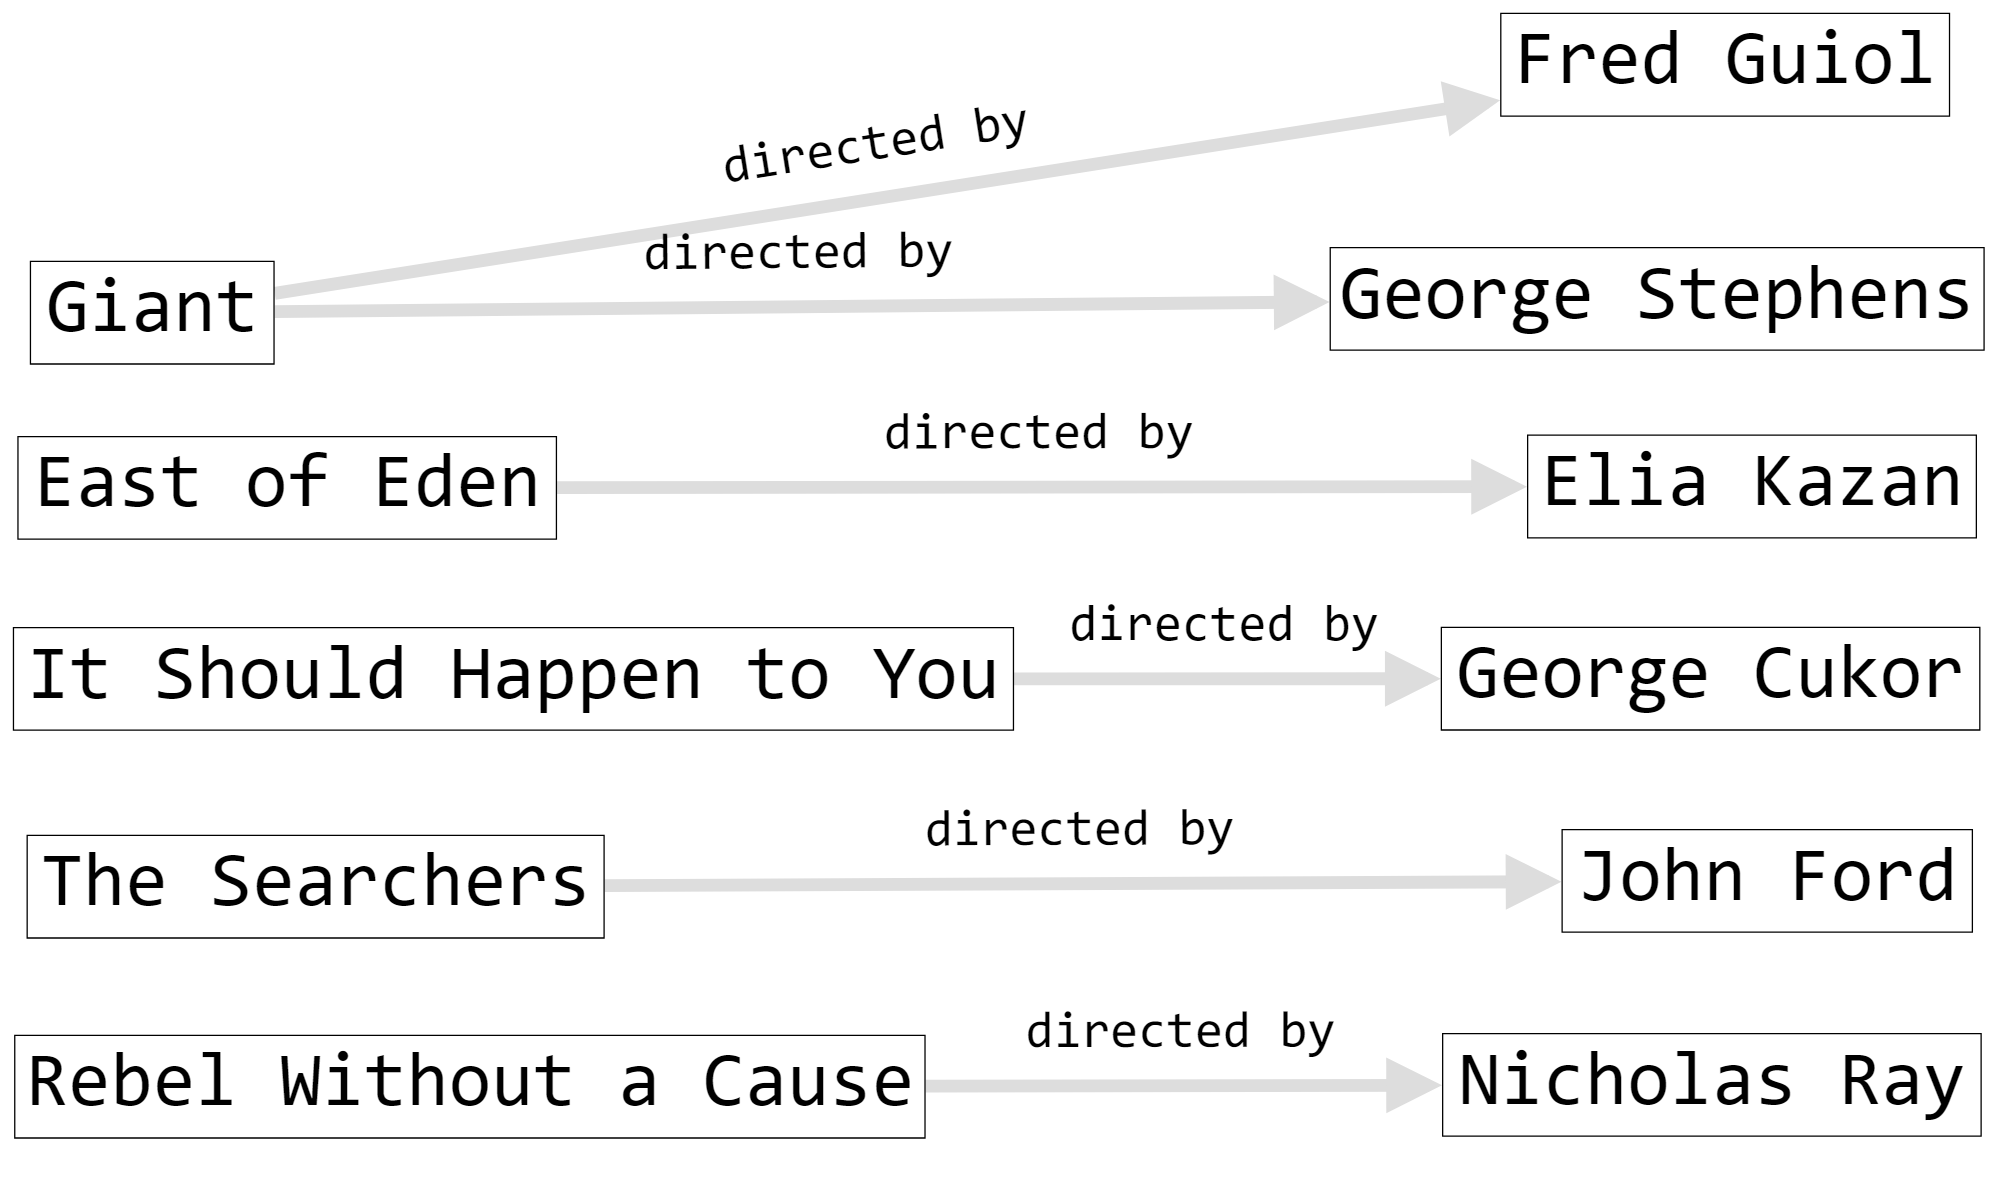
\includegraphics[width=5in]{SWWOv3/media/ch6/figure6-8a.png}
(b)
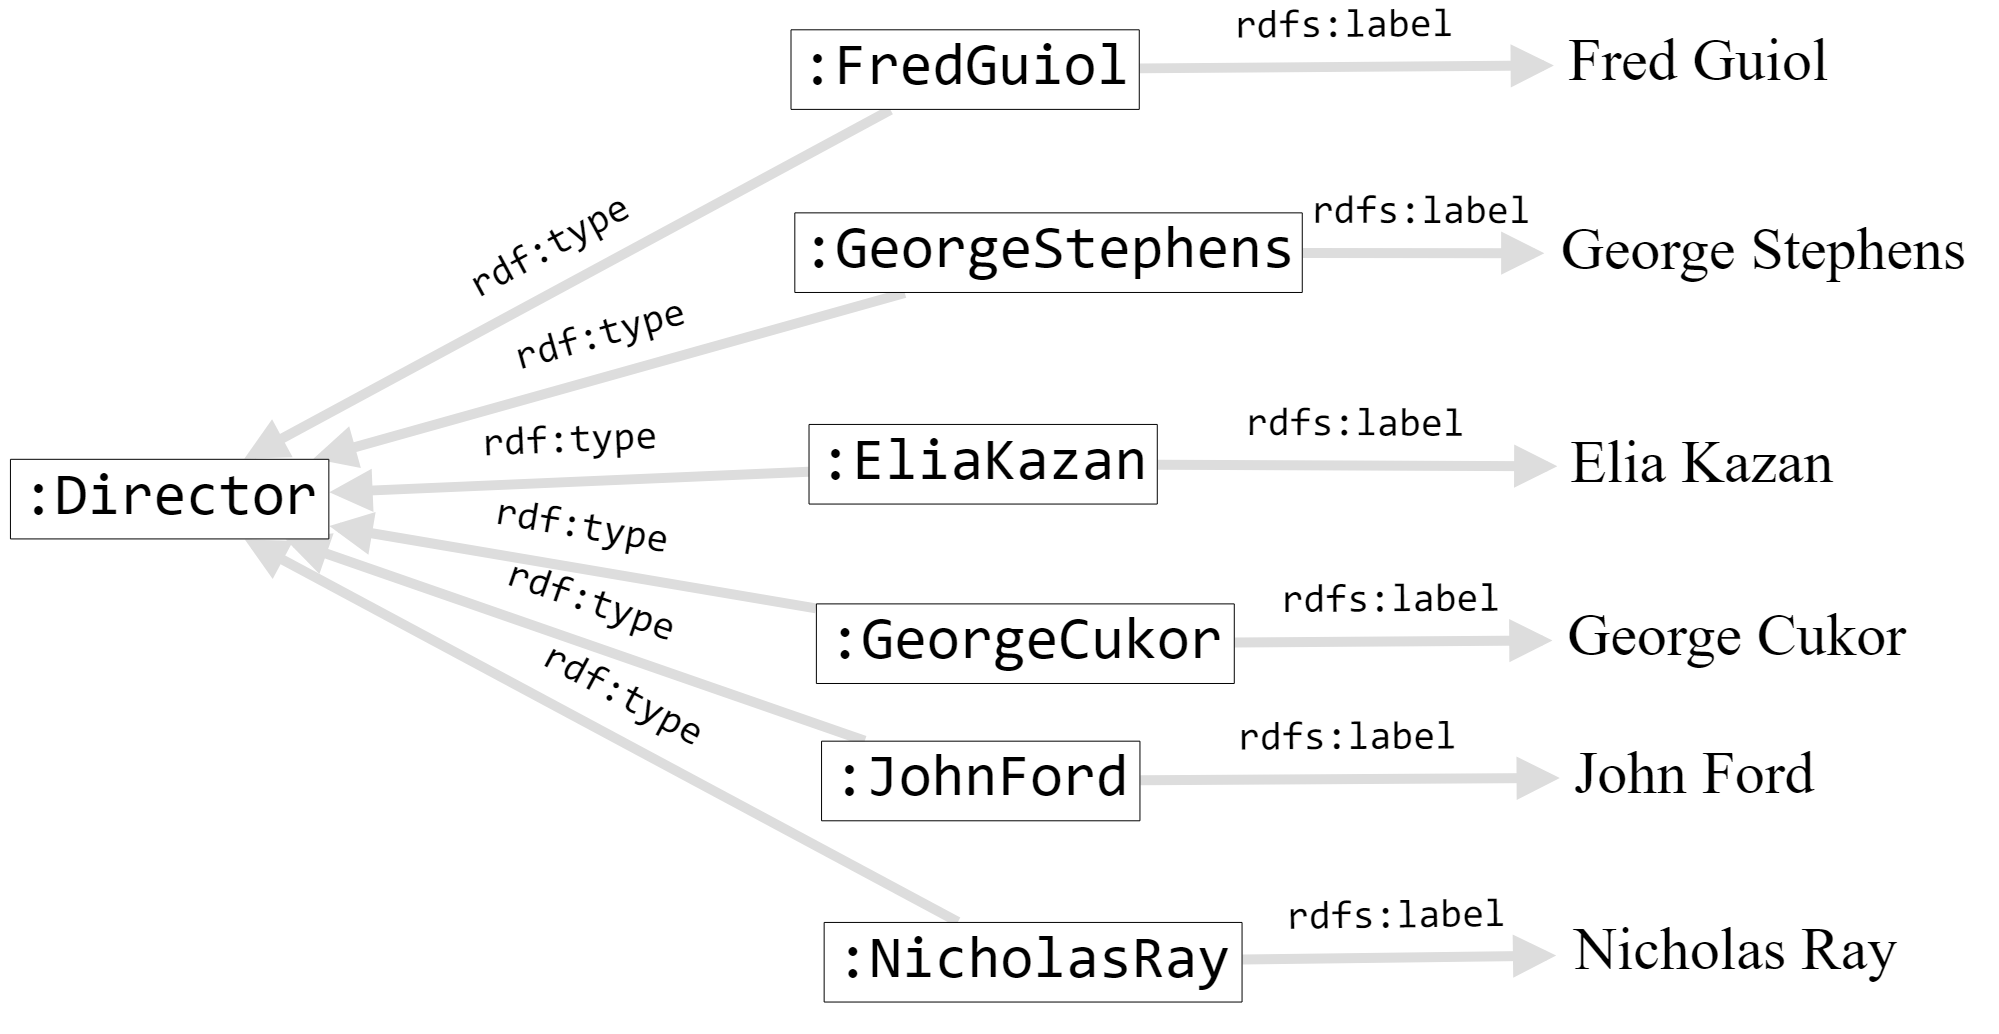
\includegraphics[width=5in]{SWWOv3/media/ch6/figure6-8b.png}
\label{fig:ch6.8}
\caption{Constructing a model about directors from a query about movies.}
\end{figure}

some data set with a SPARQL endpoint -- that is, providing a service
that responds to the SPARQL 
protocol, providing access to that data set.

\section{SPARQL Rules -- Using SPARQL as a Rule Language}

SPARQL CONSTRUCT allows us to specify templates of new information based
on patterns found in old information. A specification of this sort is
sometimes called a Rule, since it provides a way to specify things like
``Whenever you see this, conclude that.'' Examples of rules include data
completeness rules (``If John's father is Joe, then Joe's son is
John''), logical rules (``If Socrates is a man, and all men are mortal,
then Socrates is mortal''), definitions (``If Ted's sister is Maria's
mother, then Ted is Maria's uncle''), as well as business rules
(``Customers who have done more than \$5000
worth of business with us are preferred customers''). Useful rules can
often be expressed simply in 
SPARQL -- though there are some subtleties.

Consider the following data:

\begin{lstlisting}
:John a :Man.
:Joe a :Man.
:Eunice a :Woman .
:Maria a :Woman .
:Caroline a :Woman .
:Ted a :Man .
:Socrates a :Man .
:Caroline :hasFather :John .
:Ted :hasBrother :John .
:John :hasFather :Joe .
:Maria :hasMother :Eunice .
:Maria :hasFather :Sargent .
:Ted :hasSister :Eunice .
\end{lstlisting}

We could write a rule relating father to son as

\begin{lstlisting}
CONSTRUCT { ?q1 :hasSon :q2 . }
WHERE { ?q2 :hasFather ?q1 }
\end{lstlisting}

But this wouldn't quite work the way we want; while we do construct


\begin{lstlisting}
:Joe :hasSon :John .
\end{lstlisting}

as desired, we also conclude

\begin{lstlisting}
:Sargent :hasSon :Maria .
\end{lstlisting}

which is not the usual interpretation of ``son''.

So, we need to restrict the rule a bit, so that it only applies to men:

\query{A man is his father's son}
\begin{lstlisting}
CONSTRUCT ?q1 :hasSon :q2 .
WHERE { ?q2 a :Man .
        ?q2 :hasFather ?q1 }
\end{lstlisting} 


SPARQL allows us to be as specific as we want when writing a rule. The
rule about Socrates is already restricted just to men:

\begin{lstlisting}
CONSTRUCT { ?q1 a :Mortal }
WHERE { ?q1 a :Man }
\end{lstlisting}

So we will conclude that Socrates (as well as Ted, John, Joe, and
Sargent) are mortal. But Maria and 
Eunice are off the hook -- we'll draw no conclusion about them.

The definition of ``uncle'' is easy to do in SPARQL, but there are some 
things to watch out for.  For example, we might be tempted to defined it as follows: 

\begin{lstlisting}
CONSTRUCT { ?q1 :hasUncle ?q2 }
WHERE { ?q2 :hasSister ?s .
        ?q1 :hasMother ?s . }
\end{lstlisting}

This works fine to conclude that

\begin{lstlisting}
:Maria :hasUncle :Ted 
\end{lstlisting}

Since

\begin{lstlisting}
:Ted :hasSister :Eunice .
:Maria :hasMother :Eunice .
\end{lstlisting}

are both in the data set. 

But this is both too permissive and too restrictive; for example, we
won't conclude that

\begin{lstlisting}
:Caroline :hasUncle :Ted .
\end{lstlisting}

despite the fact that this is true, and follows from the data and the usual understanding of family relationships.


One way to deal with this would be to write a system of rules -- some
dealing with completeness of concepts like mother, father, sister, and
brother, and another for uncle:

\query{Rules about family relations}
\begin{lstlisting}
CONSTRUCT {?q1 :hasSibling ?q2 } WHERE {?q1 :hasBrother ?q2 }
CONSTRUCT {?q1 :hasSibling ?q2 } WHERE {?q1 :hasSister ?q2 }
CONSTRUCT {?q1 :hasParent ?q2 } WHERE {?q1 :hasFather ?q2 }
CONSTRUCT {?q1 :hasParent ?q2 WHERE {?q1 :hasMother ?q2 }
\end{lstlisting}

Now we can define uncle in terms of siblings and parents:

\query{Who's your uncle?}
\begin{lstlisting}
CONSTRUCT { ?q1 :hasUncle ?q2 }
WHERE { ?q2 :hasSibling ?parent .
        ?q2 a :Man .
        ?q1 :hasParent ?parent }
\end{lstlisting}


and can conclude both relationships:

\begin{lstlisting}
:Caroline :hasUncle :Ted .
:Maria :hasUncle :Ted .
\end{lstlisting}

(A complete model of family relationships will include quite a few data
completeness rules about siblings and parents. In Section~\ref{shacl-rules}, we'll see a
more systematic way to organize a set of rules about these things.)

If we know how much business a customer has done with us, we can write a
business rule in 
SPARQL to sort out our preferred customers.

\begin{lstlisting}
:ACME :totalBusiness 5253.00 .
:PRIME :totalBusiness 12453.00 .
:ABC :totalbusiness 1545.00 .
\end{lstlisting}

The query

\query{Preffered Customers}
\begin{lstlisting}
CONSTRUCT { ?c a :PreferredCustomer }
WHERE {?c :totalBusiness ?tb .
       FILTER (?tb > 5000)  }
\end{lstlisting}

will assert all the preferred customers:

\begin{lstlisting}
:ACME a :PreferredCustomer .
:PRIME a :PreferredCustomer .
\end{lstlisting}

Later in this section, we'll see how to use aggregators and subqueries
to compute things like total business from information about various
business transactions.

For many of these queries, it was important to restrict the application
of the query to particular sets of individuals -- e.g., Uncles and Sons
can only be Men. This is a typical sort of restriction -- a rule only
applies to a particular class of things. In Chapter 7, we'll revisit
SPARQL rules, and see how an RDFS class structure can be used to
organize a set of interacting SPARQL rules.


\begin{challenge}
\textbf{USING SPARL TO TRANSFORM HIERARCHICAL DATA}
\label{chal:2}


In the data wilderness, information comes in many forms. Some of the
variety stems from all the systems and syntaxes that we use to represent
data -- spreadsheets, XML, relational databases, and even text
documents. RDF, as a general way to represent data, resolves many of the
more superficial issues with different data formats. But even within a
single system, there are a variety of ways to represent the same
information. If we want to deal with data from the wilderness, we often
have to transform data to make it easier to use.

We'll start with a simple example. Taking some of the family tree data
from the previous example (plus a few more):

\begin{lstlisting}
:Caroline :hasFather :John .
:John :hasFather :Joe .
:Eunice :hasFather :Joe .
:Maria :hasMother :Eunice .
:Maria :hasFather :Sargent .
:Joe :hasSon :Robert .
:Joe :hasSon :Ted .
:Ted :hasSon :Patrick .
\end{lstlisting}

We could speculate about how a data set could get to be in such an
inconsistent state -- with some family relationships relating children
to their parents, while others relate parents to their children. The
data might originally come from multiple sources or have been entered
using multiple systems or by people following different methodologies.
But regardless of how it happened, this is a typical state of affairs in
the data wilderness; the data you find are organized in an inconsistent
way.

Now suppose we are interested in building a family tree that looks
something like Figure\ref{fig:ch6.9}, in which we see children and grandchildren,
regardless of gender, all in a single display. The tree is defined in a
uniform way -- Eunice has parent Joe, Maria has parent Eunice (and
Sargent), Caroline has parent John, etc.

\begin{figure}
\centering
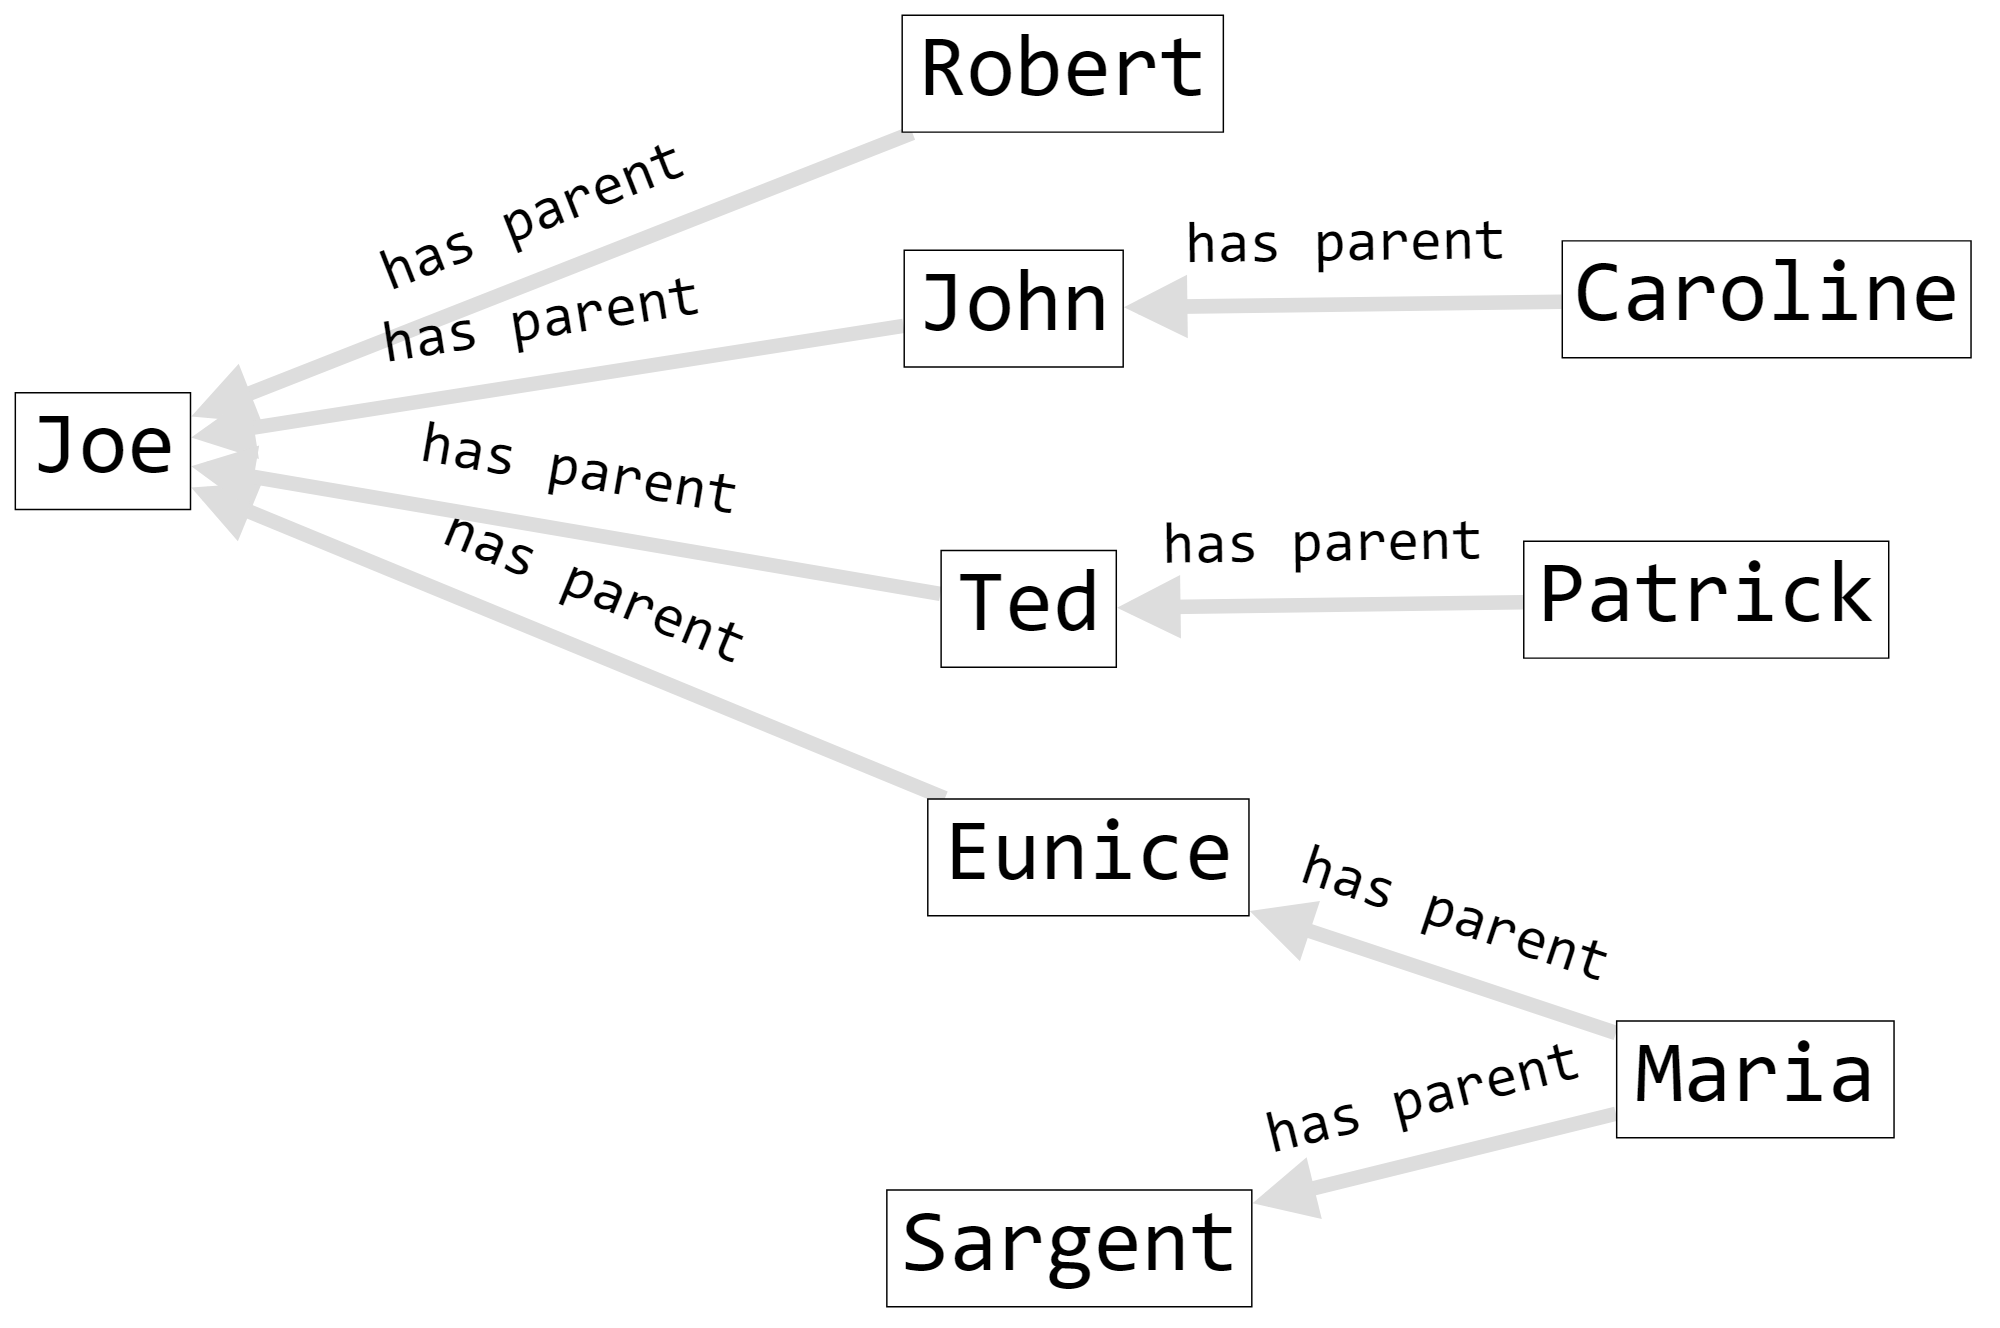
\includegraphics[width=5in]{SWWOv3/media/ch6/figure6-9.png}
\label{fig:ch6.9}
\caption{Family tree shown in a uniform manner.}
\end{figure}

All this information is available in the data set, if you abstract away
from gender words (like Son, Daughter, Mother, and Father) and re-order
some triples (turning hasSon around to be hasParent). How can we do this
using SPARQL?

We can do this by specifying a few rules as SPARQL constructs to map
these things into the form we want.

\query{Generalizing the parent relation}
\begin{lstlisting}
CONSTRUCT {?s :hasParent ?o} WHERE {?s :hasMother ?o} 
CONSTRUCT {?s :hasParent ?o} WHERE {?s :hasFather ?o} 
CONSTRUCT {?s :hasParent ?o} WHERE {?o :hasSon ?s} 
CONSTRUCT {?s :hasParent ?o} WHERE {?o :hasDaughter ?s}
\end{lstlisting}

These queries match all the various forms of hasSon, hasDaughter,
hasMother, and hasFather and map them all into appropriate triples using
hasParent. The resulting triples are


\begin{lstlisting}
:Caroline :hasParent :John .
:Eunice :hasParent :Joe .
:John :hasParent :Joe .
:Maria :hasParent :Sargent .
:Maria :hasParent :Eunice .
:Patrick :hasParent :Ted .
:Robert :hasParent :Joe .
:Ted :hasParent :Joe .
\end{lstlisting}

These provide a uniform representation of the family tree and are
amenable for producing a display like that in 
Figure\ref{fig:ch6.9}.

We can extend this example to compute the gender of the family members,
by adding another triple to each query:

\query{Generalizing the parent relation with gender}
\begin{lstlisting}
CONSTRUCT {?s :hasParent ?o .
           ?o a :Woman .}
WHERE {?s :hasMother ?o} 
CONSTRUCT {?s :hasParent ?o.
           ?o a :Man .} 
WHERE {?s :hasFather ?o} 
CONSTRUCT {?s :hasParent ?o .
           ?s a :Man .} 
WHERE {?o :hasSon ?s} 
CONSTRUCT {?s :hasParent ?o .
           ?s a :Woman .}
WHERE {?o :hasDaughter ?s}
\end{lstlisting}
\end{challenge}

\section{Transitive queries (SPARQL 1.1)}

Hierarchical data can pose very particular problems when it comes to
querying. We can see this using the example of the family tree inFigure\ref{fig:ch6.9}.
Suppose we want to query for all members of Joe's family. We can
query for his children with a simple graph pattern:

\query{Joe's children}

\begin{lstlisting}
SELECT ?member
WHERE { ?member :hasParent :Joe }
\end{lstlisting}

\textbf{\textbf{Answer:}}

\begin{tabular}{|l|}
\hline
?member\\
\hline
Eunice\\
John\\
Robert\\
Ted\\
\hline
\end{tabular}

If we want his grandchildren, we can build a slightly more complicated
query:

\query{Joe's grandchildren}

\begin{lstlisting}
SELECT ?member
WHERE {?int :hasParent :Joe .
       ?member :hasParent ?int . }
\end{lstlisting}

\textbf{\textbf{Answer:}}

\begin{tabular}{|l|}
\hline
?member\\
\hline
Maria\\
Caroline\\
Patrick\\
\hline
\end{tabular}

If we wanted Joe's great-grandchildren, we could make another query, and
so on. But what if we want all of his family, regardless of how many
generations intervene? SPARQL 1.1 includes a transitivity operator for
just this purpose. If we include a ``*'' after a property name, then the
triple matches any number of chained occurrences of the same property.

\query{Joe and his descendants}

\begin{lstlisting}
SELECT ?member
WHERE {?member :hasParent* :Joe . }
\end{lstlisting}

\textbf{\textbf{Answer:}}

\begin{tabular}{|l|}
\hline
?member\\
\hline
Joe\\
Eunice\\
Maria\\
John\\
Caroline\\
Robert\\
Ted\\
\\
Patrick\\
\hline
\end{tabular}


Notice that Joe himself is matched -- even chains of zero triples will
match. If we want to insist that there is at least one triple in the
chain (Joe's progeny, not including himself), we can use a + instead:

\query{Joe's descendants}

\begin{lstlisting}
SELECT ?member
WHERE {?member :hasParent+ :Joe . }
\end{lstlisting}

\textbf{\textbf{Answer:}}

\begin{tabular}{|l|}
\hline
?member\\
\hline
Eunice\\
Maria\\
John\\
Caroline\\
Robert\\
Ted\\
\\
Patrick\\
\hline
\end{tabular}

(SPARQL 1.1 includes a number of variations on this theme, beyond what
we cover here. Details can be found in the SPARQL 1.1 standard.)

\begin{challenge} 
\textbf{USING SPARQL TO RECORD SAMENESS IN THE LINKED MDB}
\label{chal:3}

When merging information from multiple sources, it is typical for the
same entity to appear in each data source with a different identifier.
Even in the case of a single data source, it is not unusual for the same
item to appear multiple times, with a different identifier each time.
This is especially common when the data source is implemented as a
relational database, where common practice involves separating out
information based on the role an entity plays in an application.

The Linked Movie DataBase (LinkedMDB, \cite{lmdatabase}) is an open data source containing
data about movies. The LinkedMDB is originally based on a relational database
containing information about movies, actors, directors, etc. The
underlying database includes information about what movies directors
made as well as what movies actors played in. This information is
represented in two separate tables -- a director table and an actor
table. When converted to triples, this database structure results in two
classes in the published RDF data set with corresponding names --
director and actor.

Members of the classes in the linkedMDB are given numeric URIs -- here
is a very small excerpt of data from that data set:

\begin{lstlisting}
actor:15256 
        rdf:type          film:actor ;
        film:actor_name   "Clint Eastwood" .

film:37379
       rdf:type           film:film ;
       dcterms:title      "Unforgiven" ;
       film:actor         actor:15256 ;
       film:director      director:4614 .

director:4614  
        film:director_name "Clint Eastwood" ;
        rdf:type           film:director ;
        foaf:made          film:37379 .

\end{lstlisting}

In this fragment, there is a movie whose \texttt{dcterms:title} is ``Unforgiven'' (the
namespace \texttt{dcterms} stands for ``DCMI Metadata Terms,'' a metadata standard used by
many libraries worldwide that includes standard terms for titles,
authors, publication dates, etc.), stars an actor (number 15256) whose
name is ``Clint Eastwood,'' and was directed by a director (number 4614)
whose name is ``Clint Eastwood.'' Is the fact that both of these people
are named ``Clint Eastwood'' enough for us to conclude that they are the
same person?

Fortunately, there is another triple for each of these resources in the
LinkedMBD data set:

\begin{lstlisting}
actor:15256   foaf:page  <http://www.freebase.com/view/topic/en/clint_eastwood> .
director:4614 foaf:page  <http://www.freebase.com/view/topic/en/clint_eastwood> .
\end{lstlisting}

Freebase was a linked data resource that (among other things) provided an
identity service for resources on the Web. Even though no new items are being added to Freebase
(it has been absorbed into a larger Google knowledge graph), Freebase references still provide unique
identifiers for many resources on the web. 
Any data source on the Web
can refer to a freebase URI, to unambiguously identify its own
resources. Freebase is not the only such service -- in the life
sciences, there are several such identification services for proteins,
genes, and other biological entities, and others exist for a number of
areas.  For more general use, dbpedia is a de-facto source of unique identifiers for anything that
is mentioned in wikipedia. 

In this case, we can use this information to determine that these two
people named ``Clint Eastwood'' are in fact the same person; since
linkedMDB links both of them to the same Freebase resource, they must be
the same. But what can we do with that information?

We can use SPARQL to detect identities of this sort and record it as a
new triple.

\query{Matching directors and actors}
\begin{lstlisting}
CONSTRUCT {?a skos:exactMatch ?b }
WHERE {?a foaf:page ?page .
       ?b foaf:page ?page . }
\end{lstlisting}

You can understand this query, even without knowing anything else about
the resources in it -- \texttt{foaf:page} and \texttt{skos:exactMatch} (though these will
be discussed in Sections~\ref{foaf} and Chapter~\ref{ch11}). This query simply says that any two
resources with the same \texttt{foaf:page} are \texttt{skos:exactMatch} to one another. On
this data set, we get the following triples:

\begin{lstlisting}
actor:15256 skos:exactMatch director:4614 .
director:4614 skos:exactMatch actor:15256 .
actor:15256 skos:exactMatch actor:15256 .
director:4614 skos:exactMatch director:4614 .
\end{lstlisting}

These triples indeed encode the identity match that we observed -- that
the director of \emph{Unforgiven} also played in it. But it brings along
some extra baggage -- the \texttt{exactMatch} appears twice, once relating the
actor to the director, and another time relating the director to the
actor. Furthermore, we have two rather trivial results, that every actor
is an exact match to itself (and the same for directors). These extra
results appear because SPARQL finds every match for the graph pattern in
the data; and all four bindings of \texttt{?a} and \texttt{?b} to director:4614 and
actor:15256 satisfy the pattern (they have the same values for \texttt{:page}).
These extra triples don't really cause any harm -- after all, it seems
correct to say that something is an exact match to itself -- but at the
same time, they are somewhat superfluous. In an earlier example, we were
able to drop duplicates by using the DISTINCT keyword in SPARQL. In this
case, we need something else, because  all four of these triples are
already distinct (i.e., no two have the same value for all three
positions; subject, predicate and object).

We can use a FILTER clause to eliminate many of these spurious values --
since we aren't interested in statements that say that an actor is an
exact match for himself, we can eliminate these with a filter for
matching the same values:

\query{Matching Directors vs Actors}
\begin{lstlisting}
CONSTRUCT { ?a skos:exactMatch ?b }
WHERE { ?a foaf:page ?page . 
        ?b foaf:page ?page .
        FILTER (?a != ?b) }
\end{lstlisting}

The comparison != in a filter stands for ``not equal'' -- it evaluates
to `true' just if \texttt{?a} and \texttt{?b} are not the same. This results in the
following triples:

\begin{lstlisting}
actor:15256  skos:exactMatch  director:4614 .
director:4614  skos:exactMatch  actor:15256 .
\end{lstlisting}

This is an improvement. And if we didn't know that \texttt{skos:exactMatch} is a
symmetric property (see Chapter~\ref{ch11}), we would be satisfied at this point that we had filtered out all
the spurious triples.

If we want to go one step further, we can sort these triples so that
only the first one in each pair is kept. The FILTER clause in SPARQL
includes capabilities for managing data types borrowed from XML, so
there are many ways to compare values. We can convert a URI to an XML,
then compare the strings. We can use this trick to reduce our results to
a single triple:

\query{Matching Directors to Actors 1-1}
\begin{lstlisting}
CONSTRUCT {?a skos:exactMatch ?b }
WHERE {?a foaf:page ?page .
       ?b foaf:page ?page .
       FILTER (xsd:string (?a) >  xsd:string (?b)) }
\end{lstlisting}


This query will keep a triple only when the subject comes after the
object in alphabetical order; this means that of the two triples in the
previous result, only the second one is kept:

\begin{lstlisting}
director:4614  skos:exactMatch  actor:15256 .
\end{lstlisting}

In general, there could be many ways to determine that two resources are
actually referring to the same thing; having a reference system like
Freebase or dbpedia is the easiest way. The need for such reference systems of this
kind did not begin with the Semantic Web -- it has been around for
centuries. The Semantic Web simply provides a means for publishing these
systems, and referring to them, on the Web. When there isn't a reference
system like Freebase around, more complex means of identifying
individuals can be used. The same strategy using SPARQL CONSTRUCT can be
used to determine these matches and to record them using
\texttt{skos:exactMatch}. For example, suppose that the data set included
information about date and place of birth. If it is reasonable to assume
in the data set that two people who share the same name, place, and date
of birth are indeed the same persons, then the query

\query{Match on birthplace, date, and name}
\begin{lstlisting}
CONSTRUCT {?a skos:exactMatch ?b }
WHERE {?a :name ?name ;
          :birthplace ?bplace ;
          :birthdate ?date .
       ?b :name ?name ;
          :birthplace ?bplace ;
          :birthdate ?date .
       FILTER (xsd:string (?a) >  xsd:string (?b)) }
\end{lstlisting}

will construct triples asserting the matches between these resources.

The Semantic Web doesn't provide any particular mechanism for
determining that one resource refers to the same individual as another;
it provides a means for writing down such a conclusion and publishing it
on the Web.

Now that we know that both people named Clint Eastwood are really the
same person, we are in a position to answer the question, ``Which
directors played in movies they directed?'' We can answer it with the
following query:

\query{Self-directing Actors}
\begin{lstlisting}
SELECT DISTINCT ?director
WHERE { ?dir foaf:made ?m ;
             linkedmdb:director_name ?director ;
             skos:exactMatch ?player . 
        ?m linkedmdb:actor ?player .
       }
\end{lstlisting}

\textbf{\textbf{Answer:}}

\begin{tabular}{|l|}
\hline
?director\\
\hline
``Clint Eastwood''\\
\hline
\end{tabular}
\end{challenge}

Of course, there are many other answers satisfying this condition in the full 
linkedMDB data set; we limited the output to a singleton here for simplicity. 

\begin{challenge}
\textbf{USING SPARQL TO COPY AN EXCERPT OF A DATABASE}
\label{chal:4}

An RDF data set is often made up of a very large number of triples.
There are a number of reasons why one might want to create a smaller
excerpt of such a data set:

\begin{enumerate}
\item  The data set might be available only as a network resource, with
inconsistent connectivity. You might want to keep a more robust copy of
the information that is used the most.

\item  The data set might be very large, resulting in slow query time for
complex queries. You might want to keep a cache of a small, relevant
part of the database for fast queries.

\item  The data set might contain sensitive information that should not be
disclosed to certain audiences. You might want to make a copy of the less sensitive information for public access.
\end{enumerate}


In any case, it can be useful to be able to select a part of a data set
for separate storage. This can be done with
SPARQL CONSTRUCT queries.

Following on the previous example, suppose we wanted to create a data
set that contains information about the film \emph{Unforgiven}. We want
to include the actors who played in it, its director, producer, and any
other information about it.

In the LinkedMDB, Unforgiven is given the resource name film:37379. How
can we select all the information in the LinkedMDB about Unforgiven?

Depending on just what we mean by ``all'' the information, we can start
with a simple query:

\query{Subset based on Unforgiven (Subject)}
\begin{lstlisting}
CONSTRUCT {film:37379 ?p ?o . } WHERE {film:37379 ?p ?o . }
\end{lstlisting}

This apparently trivial query selects all the triples from the data set
with film:37379 as the subject. From the full LinkedMDB, it returns a
few dozen results, including the triples:

\begin{lstlisting}
film:37379  
        rdf:type          film:film ;
        dcterms:title     "Unforgiven" ;
        film:actor        actor:25769 ;
        film:actor        actor:17281 ;
        film:director     director:4614 ;
        film:writer       writer:8240 .
\end{lstlisting}

This is a good start for getting ``all'' the information about
Unforgiven. It includes the information about actors and directors we
need to figure out that it is one of the movies that Clint Eastwood both
directed and starred in. But there could be more information in the data
set that is relevant to this movie -- for instance, there is the triple

\begin{lstlisting}
director:4614 foaf:made film:37379 .
\end{lstlisting}

This triple doesn't appear in the results of the query, since in this
case, film:37379 is the object of the triple, not the subject. We can
use a very similar query to fetch these triples:

\query{Subset based on Unforgiven (Object)}
\begin{lstlisting}
CONSTRUCT {?s ?p film:37379. } WHERE {?s ?p film:37379 . }
\end{lstlisting}

This will fetch all the triples in which \emph{Unforgiven} appears as
the object, including the \texttt{foaf:made} triple above. This is a more
comprehensive notion of what it could mean to fetch ``all'' the
information about a particular resource.

But even these triples might not seem like quite enough to tell us all
about \emph{Unforgiven}; for example, who is actor:25769? In addition to
the information about the movie itself, we might want to also identify
information about related entities. A more elaborate graph pattern can
do this as well:

\query{Larger subset based on Unforgiven}
\begin{lstlisting}
CONSTRUCT { ?s ?p ?o }
WHERE { film:37379 ?p1 ?s . }
        ?s ?p ?o . }
\end{lstlisting}

The pattern

\begin{lstlisting}
?s ?p ?o
\end{lstlisting}

matches every triple in the data set, subject to the bindings so far. In
this case, \texttt{?s} is already bound from the first triple pattern to anything
that is related (in any way) to Unforgiven. So, in this case, this
pattern copies all triples whose subjects are related to Unforgiven.

For example, since

\begin{lstlisting}
film:37379 linkedmdb:actor actor:25769 .
\end{lstlisting}

is in the data set, this query will find all the triples starting with
actor:25769, including

\begin{lstlisting}
actor:25769 film:actor_name "Richard Harris" .
\end{lstlisting}

If we merge together the results of all of these queries, we can create
a comprehensive cache of all information regarding Unforgiven. This
method was used to create many of the sample files for the examples in
this chapter.
\end{challenge}

\section{Advanced Features of SPARQL}

\subsection{Limits and ordering}

Suppose we want to know the movies that James Dean played in, and the
dates they were released:

\query{James Dean and the dates his movies were released}

\begin{lstlisting}
SELECT ?movie ?date
WHERE { :JamesDean :playedIn ?m.
        ?m rdfs:label ?movie .
        ?m dc:date ?date . }
\end{lstlisting}


\textbf{\textbf{Answer:}}

\begin{tabular}{|ll|}
\hline
?movie&?date\\
\hline
Giant&1956\\
EastOfEden&1955\\
RebelWithoutaCause&1955\\
\hline
\end{tabular}

These answers come back in no particular order; different SPARQL
implementations (and even the same implementation, at different times)
are free to produce the results in any order they like.

We can specify an ordering in the query for the results using the
directive ORDER BY. The ORDER BY directive comes after the graph pattern
and specifies one or more variables to use to determine the order in
which the results are returned. The following two examples show how this
works, ordering by 
?date and \texttt{?movie} (title), respectively:

\query{James Dean movies in release order}

\begin{lstlisting}
SELECT ?title ?date
WHERE { :JamesDean :playedIn ?movie.
        ?movie rdfs:label ?title .
        ?movie dc:date ?date . }
ORDER BY ?date
\end{lstlisting}

\textbf{\textbf{Answer:}}

\begin{tabular}{|ll|}
\hline
?title&?date\\
\hline
EastOfEden&1955\\
RebelWithoutaCause&1955\\
Giant&1956\\
\hline
\end{tabular}

\query{James Dean movies in alphabetical order}

\begin{lstlisting}
SELECT ?title ?date
WHERE { :JamesDean :playedIn ?movie.
        ?movie rdfs:label ?title .
        ?movie dc:date ?date . }
ORDER BY ?title
\end{lstlisting}

\textbf{\textbf{Answer:}}

\begin{tabular}{|ll|}
\hline
?title&?date\\
\hline
EastOfEden&1955\\
Giant&1956\\
RebelWithoutaCause&1955\\
\hline
\end{tabular}

(Note that SPARQL uses simple notions of ordering for each type of
value: numbers in numerical order, strings in alphabetic order, etc.)

Sometimes we don't want all the possible matches to a query -- for a
user interface, we might want to limit the number of items we display at
a time. Or we might want to provide a report of just the highest values
-- the ``top ten'' results. To accommodate these sorts of requests,
SPARQL includes a LIMIT directive, with which the query can specify the
maximum number of results to be fetched. LIMIT works together with ORDER
BY to determine which items to return; when LIMIT is used without ORDER
BY, the SPARQL implementation is free to fetch any matching results, up
to the specified limit.

So to find the earliest James Dean movie, we can ORDER BY ?date and
specify a LIMIT of 1:

\query{James Dean's first movie}

\begin{lstlisting}
SELECT ?title
WHERE { :JamesDean :playedIn ?m.
        ?m rdfs:label ?title .
        ?m dc:date ?date . 
ORDER BY ?date
LIMIT 1
\end{lstlisting}

\textbf{\textbf{Answer:}}

\begin{tabular}{|l|}
\hline
?title\\
\hline
East Of Eden\\
\hline
\end{tabular}

All three stars (James Dean, Natalie Wood, and Sal Mineo) of \emph{Rebel
without a Cause} died young under tragic circumstances. Which one died
first?

\query{Tragic Rebel Actors (first)}

\begin{lstlisting}
SELECT ?first
WHERE { ?who :playedIn :RebelWithoutaCause .
        ?who rdfs:label ?first .
        ?who :diedOn ?date
ORDER BY ?date
LIMIT 1
\end{lstlisting}


\textbf{\textbf{Answer:}}

\begin{tabular}{|l|}
\hline
?first\\
\hline
James Dean\\
\hline
\end{tabular}

By default, SPARQL orders results in ascending order. We can reverse the
ordering, and find the star who lived the longest with the keyword DESC
(for ``descending'')

\query{Tragic Rebel Actors (last)}

\begin{lstlisting}
SELECT ?last
WHERE { ?who :playedIn :RebelWithoutaCause ;
             rdfs:label ?last ;
             :diedOn ?date .
ORDER BY DESC (?date)
LIMIT 1
\end{lstlisting}

\textbf{\textbf{Answer:}}

\begin{tabular}{|l|}
\hline
?last\\
\hline
Sal Mineo\\
\hline
\end{tabular}

\subsection{AGGREGATES AND GROUPING (SPARQL 1.1)}

SPARQL 1.1 includes a facility for specifying aggregate functions of
data. Specifically, it provides aggregate functions COUNT, MIN, MAX,
AVG, and SUM. These aggregates can be used alongside any graph pattern,
computing a result for all matches for the pattern.

For example, we could find out how many movies James Dean has played in:

\query{How many James Dean Movies?}
\begin{lstlisting}
SELECT (COUNT (?movie) AS ?howmany)
WHERE { :JamesDean ?playedIn ?movie . }
\end{lstlisting}


The syntax of SPARQL aggregates appears in the SELECT clause -- the
aggregate expression appears in parentheses, starting with the aggregate
word, followed by the variable to be aggregated (also in parentheses),
then the keyword AS followed by a new variable, which will be bound to
the aggregated value. In this case, the query result is a single binding
for \texttt{?howmany}

\begin{tabular}{|l|}
\hline
?howmany\\
\hline
3\\
\hline
\end{tabular}

Sums work in much the same way -- suppose we want to add up the amount
of business we have done each year with various customers, and we have
data about our sales -- which company made the purchase, the amount of
the purchase, and the year in which the purchase was made. The data are
shown in tabular form here:


\begin{tabular}{|lll|}
\hline
Company&Amount&Year\\
\hline
ACME&\$1250&2010\\
PRIME&\$3000&2009\\
ABC&\$2500&2009\\
ABC&\$2800&2010\\
PRIME&\$1950&2010\\
ACME&\$2500&2009\\
ACME&\$3100&2010\\
ABC&\$1500&2009\\
ACME&\$1250&2009\\
PRIME&\$2350&2009\\
PRIME&\$1850&2010\\
\hline
\end{tabular}


As triples, each row is represented as four triples, with an arbitrary
URI for the row. Each row is a member of a single class, \texttt{:Sale}. So the
first row looks like the triples:

\query{Sales records}
\begin{lstlisting}
:row1 a :Sale ;
      :company :ACME ;
      :amount 1250 ;
      :year 2010 .
\end{lstlisting}

Using this representation in triples, we can find our total sales using
a SUM aggregator:

\query{Total sales amounts}

\begin{lstlisting}
SELECT (SUM (?val) AS ?total)
WHERE {?s a :Sale ;
          :amount ?val  }
\end{lstlisting}

\textbf{\textbf{Answer:}}

\begin{tabular}{|l|}
\hline
?total\\
\hline
24050.00\\
\hline
\end{tabular}

With this sort of data, we are interested in breaking this answer down
in various ways; how much business did we do with each customer? How
much business did we do in a given year? SPARQL allows us to organize
the query in these ways, using the notion of GROUP BY. For instance, we
can find the amount of business for each year by grouping by years:

\query{Total sales amounts by year}

\begin{lstlisting}
SELECT ?year (SUM (?val) AS ?total)
WHERE { ?s a :Sale ;
           :amount ?val ;
           :year ?year  }
GROUP BY ?year
\end{lstlisting}

\textbf{\textbf{Answer:}}

\begin{tabular}{|ll|}
\hline
?year&?total\\
\hline
2009&13100.00\\
2010&10950.00\\
\hline
\end{tabular}

The GROUP BY keyword comes after the graph pattern and informs the
aggregate how to group the sums; instead of summing all the results, it
sums results grouped by the specified variable. In this case, the sum is
grouped by \texttt{?year}. The GROUP BY variable must already have been bound in
the graph pattern; these values are used to sort the results for
aggregation. Since a variable mentioned in the GROUP BY clause will have
the same value for every summand for a particular sum, it is sensible to
include it in the SELECT clause (if desired). Other variables (like \texttt{?s}
and \texttt{?val}) will have different values for each summand, and hence won't
have a single defined value for a sum; these variables are not available
for inclusion in the SELECT clause.

We can sort by more than one variable at a time:

\query{Total sales amounts by company per year}

\begin{lstlisting}
SELECT ?year ?company (SUM (?val) AS ?total)
WHERE { ?s a :Sale ;
           :amount ?val ;
           :year ?year ;
           :company ?company . }
GROUP BY ?year ?company
\end{lstlisting}

\textbf{\textbf{Answer:}}

\begin{tabular}{|lll|}
\hline
?year&?company&?total\\
\hline
2009&ACME&3750.00\\
2009&ABC&4000.00\\
2009&PRIME&5350.00\\
2010&ACME&4350.00\\
2010&PRIME&3800.00\\
2010&ABC&2800.00\\
\hline
\end{tabular}

This tells us how much business we did with each customer in a
particular year. If we'd like to find out customers that did more than
\$5000 of business in some year, we can show only some of these results,
using the keyword HAVING to choose particular results:

\query{Top companies by sales amounts}

\begin{lstlisting}
SELECT ?year ?company (SUM (?val) AS ?total)
WHERE { ?s a :Sale ;
           :amount ?val ;
           :year ?year ;
           :company ?company . }
GROUP BY ?year ?company
HAVING (?total  5000)
\end{lstlisting}

\textbf{\textbf{Answer:}}

\begin{tabular}{|lll|}
\hline
?year&?company&?total\\
\hline
2009&PRIME&5350.00\\
\hline
\end{tabular}

PRIME was the only customer who satisfied this criterion, which they did
in 2009. The keywords HAVING and FILTER are very similar; both of them
introduce a condition that is to be met by the results. FILTER refers to
variables bound within a particular graph pattern, hence the FILTER
keyword always appears in the pattern (between ``\{`` and ''\}''), while
HAVING refers to variables defined by aggregations in the SELECT clause,
and hence always appears outside a graph pattern.

\subsection{Subqueries (SPARQL 1.1)}

A subquery is a query within a query. Since a SPARQL graph pattern can
include arbitrary connections between variables and resource
identifiers, there isn't as much need to have subquery as there is in
other query languages. In fact, for basic SPARQL (i.e., without limit or
aggregate functions), there is no need for subquery at all.

But subqueries can be useful when combining limits and aggregates with
other graph patterns. A question has to be pretty complex to require a
subquery in SPARQL. A subquery limits the scope of things like
aggregators, orderings, and limits to just part of the query. Following
along the example using customer sales above, we notice that some
companies increased their sales from 2009 to 2010, while others
decreased. We can use subqueries to find out which ones increased their
sales during that time:

\query{Comparative sales year to year}

\begin{lstlisting}
SELECT ?company
WHERE {
    {SELECT ?company ((SUM(?val)) AS ?total09)
     WHERE {
            ?s a :Sale ;
               :amount ?val ;
               :company ?company ;
               :year 2009 .  }
     GROUP BY ?company  . }
    {SELECT ?company ((SUM(?val)) AS ?total10)
     WHERE {
            ?s a :Sale ;
               :amount ?val ;
               :company ?company ;
               :year 2010 . }
     GROUP BY ?company  . }
    FILTER (?total10  ?total09) .
}
\end{lstlisting}
\textbf{\textbf{Answer:}}

\begin{tabular}{|l|}
\hline
?company\\
\hline
ACME\\
\hline
\end{tabular}

The two subqueries in this example compute the total sales for years
2009 and 2010, respectively. The FILTER retains only the matches in
which the 2010 total exceeds the 2009 totals -- customers who did more
business in 2010 than in 2009. Each subquery (including GROUP BY etc. at
the end) is enclosed in braces. Within the subqueries, variables have
their own scope; that is, the variable \texttt{?val} in each of these subqueries
matches completely different values (in one subquery, it matches the
2009 values; in the other, it matches the 2010 values). This sort of
computation requires subqueries, since it involves independent subsets
of the data to be compared.

Another application of subqueries is to bring the power of aggregates
(available only in SELECT queries) to other SPARQL query constructs
(like ASK and CONSTRUCT). Earlier, we saw a query that selected the
companies who had done more than \$5000 worth of business in a single
year.

Suppose we wanted to use this result as part of a CONSTRUCT query --
where would we put the aggregation specification? This can be handled
uniformly with a subquery, as in the following example:

\query{Preferred Customers}
\begin{lstlisting}
CONSTRUCT { ?company a :PreferredCustomer.
            ?company :totalSales ?total . }
WHERE {SELECT ?year ?company (SUM (?val) as ?total)
       WHERE { ?s a :Sale ;
                  :amount ?val ;
                  :year ?year ;
                  :company ?company . }
       GROUP BY ?year ?company 
       HAVING (?total  5000)
      }
\end{lstlisting}


This results in two triples:

\begin{lstlisting}
:PRIME a :PreferredCustomer . 
:PRIME :totalSales 5350.00 .
\end{lstlisting}


The subquery is the same query we saw before, determining which
companies did more than \$5000 of business in a single year. The
CONSTRUCT query creates a graph with just the information about
preferred customers -- their preferred status as membership in the class
\texttt{:PreferredCustomer}, and the total sales as a numeric value.

\subsection{UNION}

A graph pattern is made up of several triples -- all of which have to
match in order for the pattern to match. In logical terms, this means
that there is an implicit ``and'' operation between the triples. One
could correctly read a graph pattern as saying ``the first triple
matches AND the second triple matches AND the third triple matches .''
But there are times when we might want to say that this triple matches
OR that triple matches. For those times, SPARQL provides UNION.

UNION combines two graph patterns, resulting in the set union of all
bindings made by each pattern. Variables in each pattern take values
independently (just as they do in subqueries), but the results are
combined together.

A simple example would be to find out all the actors who played either
in \emph{Rebel without a Cause} or
\emph{Giant}. Each of these is a simple query; we can get all the
answers by making a UNION of the two queries:

\query{Actors in Rebel or Giant}

\begin{lstlisting}
SELECT ?actor
WHERE {
        {?actor :playedIn :Giant .}
        UNION
        {?actor :playedIn :RebelWithoutaCause . }
      }
\end{lstlisting}


\textbf{\textbf{Answer:}}

\begin{tabular}{|l|}
\hline
actor\\
\hline
Ann Doran\\
Carroll Baker\\
Elizabeth Taylor\\
James Dean\\
James Dean\\
Jim Backus\\
Mercedes McCambridge\\
Natalie Wood\\
Rock Hudson\\
Sal Mineo\\
Sal Mineo\\
\hline
\end{tabular}

Some names appear twice, if the actor appeared in both movies. This
repetition can be removed by using the DISTINCT keyword.

UNION can be used in the context of CONSTRUCT as well. In a challenge
earlier in this chapter, we used SPARQL to transform hierarchical
information, by mapping several related relationships (mother, father,
son, daughter) onto a single hierarchy (parent); the resulting triples
were shown in Figure\ref{fig:ch6.9}. This involved four CONSTRUCT queries, with an
implicit understanding that all the triples resulting from each query
would be merged. This is a perfectly fine assumption, if the queries are
run in the context of a program that indeed combines all the results
(e.g., by adding all the triples to the same triple store). But with
UNION, we can specify explicitly that the triples are to be combined. We
can take the graph pattern for each of the triples, and combine them all
with the UNION operator, thus:

\query{Combining types of parenthood}
\begin{lstlisting}
CONSTRUCT {?s :hasParent ?o}
WHERE{ {?s :hasMother ?o}
       UNION
       {?s :hasFather ?o}
       UNION
       {?o :hasSon ?s}
       UNION
       {?o :hasDaughter ?s}
     }
\end{lstlisting}

The result of this query is the same as the combined results of the
queries in the Challenge, i.e., the set of hasParent relationships shown
in Figure~\ref{fig:ch6.9}.

\subsection{Assignments (SPARQL 1.1)}
\label{assignments}

Suppose we want to query the full names of the authors of the book
``Semantic Web for the Working Ontologist.'' We can easily find first
names and last names, but how do we get the full names? It is a simple
enough computation -- concatenate the first and last names together,
with an embedded space. But the string ``James Hendler'' is nowhere to
be found in the data set. How do we create it?

Tell-and-ask systems typically answer questions based on information
that was told to them -- this is true for spreadsheets, notebooks,
databases, and RDF stores. But many tell-and-ask systems go
beyond this, and provide ways for you to specify information that you
didn't (directly) tell the system. We have already seen how this can be
done with aggregators in SPARQL -- the sums, averages, counts, etc., are
information that was not directly told to the system, but was computed
from information that was already there.

But sometimes we would like to specify a special purpose computation as
part of the \emph{ask} process. Spreadsheets excel at this functionality, with
the ability for the user to specify arbitrary formulas that will be
calculated and updated whenever data are changed or entered. Databases
have stored procedures that execute arbitrary code based on information
in the database. SPARQL provides a similar capability through query-time
assignments. An assignment lets the query write specifically the value
of a variable through some computation -- ``assigning'' a value to that
variable, rather than matching some value in the data.

Assignments are not supported in the SPARQL 1.0 standard but are
supported in the 1.1 standard. Assignments are expressed with the
keyword BIND,  as follows:

\begin{lstlisting}
BIND ( expression (...) AS ?var)
\end{lstlisting}

The expression can include arithmetic formulas (using the usual
operators +. -. *, /, etc.) or a series of function calls, and references to other variables
that have already been matched or bound. Like stored
procedures in relational databases, the function calls can include
arbitrary programs in a variety of programming languages. For the
examples in this book, we will restrict ourselves to some standard
functions, those from the XPATH specification for XML.

Suppose we have some data about books and their authors, including the
following data:

\begin{lstlisting}
:DeanAllemang rdf:type :Person ;
              :firstName "Dean" ;
              :lastName "Allemang" .

:JimHendler rdf:type :Person ;
            :firstName "James" ;
            :lastName "Hendler" .

:FabienGandon rdf:type :Person ;
              :firstName "Fabien" ;
              :lastName "Gandon" .

:WorkingOntologist rdf:type :Book ;
    rdfs:label "Semantic Web for the Working Ontologist" ;
    dc:creator :DeanAllemang , :JimHendler, :FabienGandon .
\end{lstlisting}


This is where assignments come in. We can match for the first and last
names, but we need to do a computation to get the full name. There is a
function for concatenate in SPARQL - it is called CONCAT. We
can use this to compute the full names:

\query{Full names of Authors}

\begin{lstlisting}
SELECT ?fullname
WHERE { :WorkingOntologist dc:creator ?author .
        ?author :firstName ?first .
        ?author :lastName ?last . 
        BIND (CONCAT (?first, " ", ?last) AS ?fullname)}
\end{lstlisting}


\textbf{\textbf{Answer:}}

\begin{tabular}{|l|}
\hline
?fullname\\
\hline
James Hendler\\
Dean Allemang\\
Fabien Gandon\\
\hline
\end{tabular}

Assignments are a convenient way to compute information based on other
things you are already asking for. But they really show their power when
they are used for intermediate computations, so that the results of an
assignment can be used to specify parameters for the ongoing search.

As an example, let's consider merging the information about this book
with our movie database. One might wonder if there are any actors with
names that are like the authors of this book -- perhaps one whose name
is made up of the first names of the book's authors. We can fetch those
first names easily enough:

\query{Combined first names of Authors}

\begin{lstlisting}
SELECT ?n1 ?n2
WHERE { authors:WorkingOntologist dc:creator ?a1 .
        authors:WorkingOntologist dc:creator ?a2 .
        ?a1 authors:firstName ?n1 .
        ?a2 authors:firstName ?n2 . }
\end{lstlisting}

\textbf{\textbf{Answer:}}

\begin{tabular} {|ll|}
\hline
?n1&?n2\\
\hline
Dean&Dean\\
Dean&James\\
Dean&Fabien\\
James&Dean\\
James&Fabien\\
James&James\\
Fabien&Dean\\
Fabien&James\\
Fabien&Fabien\\
\hline
\end{tabular}

Now, let's make a full name out of the two first names, by concatenating
them together, using the same function from XPATH as in the previous
example. At the same time, we'll get rid of the situations where both
variables match the same name by filtering them out. This leaves us
with:

\query{Combined first names as a search probe}

\begin{lstlisting}
SELECT ?probe
WHERE { authors:WorkingOntologist dc:creator ?a1 .
        authors:WorkingOntologist dc:creator?a2 .
        ?a1 authors:firstName ?n1 .
        ?a2 authors:firstName ?n2 .
        FILTER (?a1 != ?a2)
        BIND (CONCAT (?n1, " ", ?n2) AS ?probe)
      }

\end{lstlisting}


\textbf{\textbf{Answer:}}

\begin{tabular} {|l|}
\hline
?probe\\
\hline
``Dean James''\\
``Dean Fabien''\\
``James Dean''\\
``James Fabien''\\
``Fabien Dean''\\
``Fabien James''\\
\hline
\end{tabular}

Now, let's use this computed result as a way to query the movie
database. We want to find an actor who has one of these as his name. If
we consider an actor to be someone who acts in a movie, we can find such
an actor by matching a triple for the predicate \texttt{:playsIn}.

\query{Actors with names like the Authors}

\begin{lstlisting}
SELECT DISTINCT ?who
WHERE {
       authors:WorkingOntologist dc:creator ?a1 . 
       authors:WorkingOntologist dc:creator ?a2 .
       ?a1 authors:firstName ?n1 .
       ?a2 authors:firstName ?n2 .
       FILTER (?a1 != ?a2)
       BIND (CONCAT (?n1, " ", ?n2)) AS ?probe)
       ?who movies:playedIn ?any .
       ?who rdfs:label ?probe .
      }
\end{lstlisting}


\textbf{\textbf{Answer:}}

\begin{tabular}{|l|}
\hline
?who\\
\hline
movies:JamesDean\\
\hline
\end{tabular}

Indeed, there is an actor in the database whose full name is made up of
the concatenation of the first names of authors of this book.

\subsection{Data in queries}
\label{sparqlvalues}

Normally, we expect a query to get its data from a data source.  Sometimes it 
is convenient to include small bits of data right in the query itself.  For example, we 
could have a small data set that incudes the names of the authors of this book, as we did in 
Section~\ref{assignments}.  Alternatively, we could just list those names 
as part of the query itself, since there aren't many data and we can just as easily
list them: 




\query{Including author names in the query}
\begin{lstlisting}
SELECT * 
WHERE  {
    VALUES (?firstname ?lastname) {("James" "Hendler")
    ("Dean" "Allemang")
    ("Fabien" "Gandon")}
    BIND (CONCAT (?firstname, " ", ?lastname) AS ?fullname)
}
\end{lstlisting}

\textbf{\textbf{Answer:}}

\begin{tabular}{|lll|}
\hline
?firstname&?lastname&?fullname\\
\hline
James&Hendler&James Hendler\\
Dean&Allemang&Dean Allemang\\
Fabien&Gandon&Fabien Gandon\\
\hline
\end{tabular}



\subsection{Federating SPARQL Queries}

In the previous example, we assumed that all the triples about books and
authors, and the triples about movies were available in a single graph.
This isn't such a far-fetched assumption, since it is a conceptually
simple matter to merge multiple graphs into a single one for the purpose
of running queries. But it is certainly not guaranteed that this will be
the case; when data sets are very large, it can be impractical to merge
them together before querying them. The data sets may be available only
on the Web, and access to them could be limited.

For this reason, it is desirable to be able to federate a query across
more than one data source. ``Federate'' in this sense means to virtually
combine the data sources in the query, while leaving each component with
its own identity. Multiple data sources can be made available in a
variety of ways. Data sources on the Web can be published for remote
access as SPARQL endpoints. But even within a single data source, sets
of triples can be given names as named graphs. Both endpoints and named
graphs can participate in federated SPARQL queries.

When each data set is published via a SPARQL endpoint, SPARQL allows
subqueries to be dispatched to different endpoints. The endpoint for the subquery is
specified by putting the keyword SERVICE followed by a URL for the
SPARQL endpoint before a graph pattern. A similar syntax is used for
named graphs, but using the keyword GRAPH, followed by the URL that
denotes the named graph. For instance, we could find out what the SPARQL
endpoint dbpedia
\href{http://dbpedia.org/sparql)}{(http://dbpedia.org/sparql)} knows
about the movies that James Dean played in. As a simple query, we could
find out whether there are any entries in dbpedia that have labels
matching the names of actors who played in the movie \emph{Giant}:

\query{Federating with dbpedia.org}
\begin{lstlisting}
SELECT ?entry
WHERE {?actor :playedIn :Giant .
       ?actor rdfs:label ?name . 
       SERVICE <http://dbpedia.org/sparql>
           {?entry rdfs:label ?name . }
      }
\end{lstlisting}


\textbf{\textbf{Answer:}}

\begin{tabular}{|l|}
\hline
?entry\\
\hline
http://dbpedia.org/resource/Carroll\_Baker\\
http://dbpedia.org/resource/Elizabeth\_Taylor\\
http://dbpedia.org/resource/James\_Dean\\
http://dbpedia.org/resource/Mercedes\_McCambridge\\
http://dbpedia.org/resource/Rock\_Hudson\\
http://dbpedia.org/resource/Sal\_Mineo\\
\hline
\end{tabular}

The variable \texttt{?name}, which was defined in the second triple, is used
again in the subquery; in effect, a value from the local data set has
been given to the remote data set (dbpedia) as a pre- defined binding of
a variable. From the point of view of the dbpedia endpoint, \texttt{?name} isn't
a variable anymore; it is already bound to some value(s) from outside
the query (``\emph{Giant},'' ``\emph{Rebel without a Cause},'' and
``\emph{East of Eden}''). The value(s) found for \texttt{?entry} in the subquery
is available as a result for the full query.

The query we made to the dbpedia service in this example wasn't very
interesting -- it just found the dbpedia reference for something
(someone) we already know about. It would be more interesting

if we would ask dbpedia to tell us something we don't already know --
for instance, the birth name of these actors:

\query{Birth names of actors in Giant}

\begin{lstlisting}
SELECT DISTINCT ?name ?realname
WHERE {?actor :playedIn :Giant .
       ?actor rdfs:label ?name .
       SERVICE
           <http://dbpedia.org/sparql{http://dbpedia.org/sparql>
           { ?entry rdfs:label ?name .
             ?entry dbpedia:birthname ?realname  }
      }
\end{lstlisting}


\textbf{\textbf{Answer:}}

\begin{tabular}{|ll|}
\hline
?name&?realname\\
\hline
Elizabeth Taylor&Elizabeth Rosemond Taylor\\
Rock Hudson&Roy Harold Scherer, Jr.\\
Sal Mineo&Salvatore Mineo, Jr.\\
\hline
\end{tabular}

A drawback of this query is that it assumes that \texttt{rdfs:label} is an
appropriate property for identifying a resource in dbpedia. But dbpedia
has information about millions of things -- people, movies, places,
countries, etc. It includes pretty much anything that has a Wikipedia
entry; it is likely that two things could have the same \texttt{rdfs:label}. A
better way to identify a resource in dbpedia would be to refer to the
dbpedia URL directly. This isn't something we can just do in the query
-- the data source would have to include a link between its resources
and dbpedia. For example, if the data source were to include the
following triples:

\begin{lstlisting}
:ElizabethTaylor skos:exactMatch dbpedia:Elizabeth_Taylor .
:RockHudson skos:exactMatch dbpedia:Rock_Hudson .
:SalMineo skos:exactMatch dbpedia:Sal_Mineo .
\end{lstlisting}

then we could change the query to be 

\query{Birth names of actors in Giant (exact match)}
\begin{lstlisting}
SELECT DISTINCT ?name ?realname
WHERE {?actor :playedIn :Giant .
       ?actor skos:exactMatch ?db .
       SERVICE <http://dbpedia.org/sparql>
           { ?db dbpedia:birthname ?realname }
      }
\end{lstlisting}

Not only is this a shorter query, but it also has less chance of going
awry; even if there are other people with names like ``Sal Mineo'' or
``Elizabeth Taylor,'' the inclusion of the exact match in the data set
ensures that the correct resource will be used in the dbpedia query.
This use of exactMatch is an example of the practice we recommended in
chapter\ref{ch5}, to link data across data set to weave a Web of linked data.
It has become quite common for published data sets to include this sort
of linkage to data source like dbpedia to resolve ambiguity -- dbpedia
has become a \emph{de facto} registry of names for celebrities, places,
works of art, etc., that is, for anything that is mentioned in
Wikipedia.

Any number of federated SERVICE specifications are allowed in a SPARQL
query, making it possible to write queries that are federated over
several data sources.

\section{SUMMARY}

The SPARQL query language provides a means for querying information from
an RDF data graph. The workhorse of the query is the graph pattern -- a
smaller graph including both resources and variables, that is matched
against a data graph. The graph pattern specifies what information is to
be fetched from the graph, and how the entities that match the variables
are related to one another.

SPARQL queries can be used to fetch information (like SQL queries) or to
transform a graph into a new form (like rules). Both forms use the same
notion of graph pattern to specify the desired information.

\subsection{Fundamental concepts}

The following fundamental concepts were introduced in this chapter.

Graph pattern -- a graph with wildcards, used to match against a data
graph to specify desired results.

Variables (question words) -- wildcards in a graph pattern. They can
match any resource.

\textbf{SELECT} query -- a query form that fetches binding for variables from a
graph.

CONSTRUCT query -- a query form that builds a new graph based on matches
in a data graph, along with a graph template.

Queries as rules -- using a CONSTRUCT query to specify rules.

Federated query -- querying multiple data sources in a single query.

